%---------------------------------------------------------------------------%
%-                                                                         -%
%-                           LaTeX Template                                -%
%-                                                                         -%
%---------------------------------------------------------------------------%
%- Copyright (C) Huangrui Mo <huangrui.mo@gmail.com> 
%- This is free software: you can redistribute it and/or modify it
%- under the terms of the GNU General Public License as published by
%- the Free Software Foundation, either version 3 of the License, or
%- (at your option) any later version.
%---------------------------------------------------------------------------%
%->> Document class declaration
%---------------------------------------------------------------------------%
\documentclass[twoside]{Style/ucasthesis}%
%- Multiple optional arguments:
%- [<oneside|twoside|print>]% oneside eprint, twoside eprint, or paper print
%- [fontset=<adobe|none|...>]% specify font set instead of automatic detection
%- [scheme=plain]% thesis writing of international students
%- [draftversion]% show draft version information
%- [standard options for ctex book class: draft|paper size|font size|...]%
%---------------------------------------------------------------------------%
%->> Document settings
%---------------------------------------------------------------------------%
\usepackage[authoryear,list]{Style/artratex}% document settings
%- usage: \usepackage[option1,option2,...,optionN]{artratex}
%- Multiple optional arguments:
%- [bibtex|biber]% set bibliography processor and package
%- [<numbers|super|authoryear|alpha>]% set citation and reference style
%- <numbers>: textual: Jones [1]; parenthetical: [1]
%- <super>: textual: Jones superscript [1]; parenthetical: superscript [1]
%- <authoryear>: textual: Jones (1995); parenthetical: (Jones, 1995)
%- <alpha>: textual: not available; parenthetical: [Jon95]
%- [geometry]% reconfigure page layout via geometry package
%- [lscape]% provide landscape layout environment
%- [xhf]% disable header and footer via fancyhdr package
%- [color]% provide color support via xcolor package
%- [background]% enable page background
%- [tikz]% provide complex diagrams via tikz package
%- [table]% provide complex tables via ctable package
%- [list]% provide enhanced list environments for algorithm and coding
%- [math]% enable some extra math packages
%- [xlink]% disable link colors
\usepackage{Style/artracom}% user defined commands
%---------------------------------------------------------------------------%
%->> Document inclusion
%---------------------------------------------------------------------------%
%\includeonly{Tex/Chap_1,...,Tex/Chap_N}% selected files compilation
%---------------------------------------------------------------------------%
%->> Document content
%---------------------------------------------------------------------------%
%-
%-> Titlepage information
%-
%---------------------------------------------------------------------------%
%->> Titlepage information
%---------------------------------------------------------------------------%
%-
%-> 中文封面信息
%-
\confidential{}% 密级:只有涉密论文才填写
\schoollogo[scale=0.095]{ucas_logo}% 校徽
\title{基于语义地图的增强现实虚实融合关键技术研究}% 论文中文题目
\author{张琪}% 论文作者
\advisor{蒋永实~研究员~中国科学院自动化研究所\\朱晓阳~副研究员~中国科学院自动化研究所\\于海涛~副研究员~中国科学院自动化研究所}% 指导教师:姓名 专业技术职务 工作单位
%\advisor{指导教师一\\指导教师二\\指导教师三}% 多行指导教师示例
\degree{硕士}% 学位:学士、硕士、博士
\degreetype{工学}% 学位类别:理学、工学、工程、医学等
\major{虚拟现实与人机交互}% 二级学科专业名称
\institute{中国科学院自动化研究所}% 院系名称
%\institute{中国科学院力学研究所\\流固耦合实验室}% 多行院系名称示例
\date{2020~年~6~月}% 毕业日期:夏季为6月、冬季为12月
%-
%-> 英文封面信息
%-
\TITLE{A Research on Key Technologies of Augmented Reality Fusion Based on Semantic Map}% 论文英文题目
\AUTHOR{Qi Zhang}% 论文作者
\ADVISOR{Supervisor: \\Professor Yongshi Jiang\\Associate Professor Xiaoyang Zhu\\Associate Professor Haitao Yu}% 指导教师
\DEGREE{Master}% 学位:Bachelor, Master, Doctor, Postdoctor。封面据英文学位名称自动切换,需确保拼写准确
\DEGREETYPE{Engineering}% 学位类别:Philosophy, Natural Science, Engineering, Economics, Agriculture 等
\MAJOR{Virtual Reality and Human-Computer Interaction}% 二级学科专业名称
\DATE{June, 2020}% 毕业日期:夏季为June、冬季为December
%---------------------------------------------------------------------------%
%
\begin{document}
%-
%-> Frontmatter: title page, abstract, content list, symbol list, preface
%-
\frontmatter% initialize the environment
%---------------------------------------------------------------------------%
%->> Frontmatter
%---------------------------------------------------------------------------%
%-
%-> 生成封面
%-
\maketitle% 生成中文封面
\MAKETITLE% 生成英文封面
%-
%-> 作者声明
%-
\makedeclaration% 生成声明页
%-
%-> 中文摘要
%-
\intobmk\chapter*{摘\quad 要}% 显示在书签但不显示在目录
\setcounter{page}{1}% 开始页码
\pagenumbering{Roman}% 页码符号

增强现实是一种将虚拟信息通过虚实融合技术叠加显示到真实场景恰当位置处,以此提升用户与真实环境之间的交互体验的技术,它
广泛应用于科普教育、军事仿真、文化旅游、医养健康、装备维保等众多领域。虚实融合技术是增强现实领域的关键技术之一,
它通过跟踪相机自身位姿,将虚拟资料在环境中准确注册,直接影响了系统的真实性体验。
基于特征的视觉SLAM技术能一定程度上解决相机位姿估计和环境几何信息理解的问题,从而帮助虚实融合,
但在动态环境下的位姿估计和建图性能、语义信息表达能力等方面仍有不足。本文针对以上问题,构建了结合深度神经网络和视觉SLAM框架的语义SLAM系统,
对于对动态场景下位姿估计优化方法、语义地图的构建和表示方法及在增强现实系统中的应用方法进行了研究。本文的主要工作和贡献如下:
{
\setlist[enumerate]{}% restore default behavior
\begin{enumerate}[nosep]
    \item 针对动态场景下基于特征的视觉SLAM方法相机位姿估计精度低的问题,提出了双阶段的动态外点滤除算法。此算法结合基于语义类别的
    自适应权重生成方法和基于极线约束的动态一致性检测方法,能够对于不同类别的物体自适应生成不同的判定条件,判断其是否处于运动状态,
    并移除处于运动状态的物体的轮廓内的特征点。此算法在TUM RGB-D数据集上进行了验证,在动态场景下其结果比ORB-SLAM2有数量级式的提升,
    提升幅度在大部分指标上优于业界先进系统,表明它能够有效提升基于特征的视觉SLAM系统在动态场景下的位姿估计精度和鲁棒性。
    \item 针对现有方法缺乏对环境高层语义理解导致虚实融合真实感不强的问题,分别探究了基于局部特征的预置语义库地图和语义SLAM系统生成的
    物体级三维语义点云地图的构建和表示方法。对于预置语义库地图提出了特征识别和跟踪方法,验证了其对室外环境的表示能力和在增强现实导航系统中的应用能力。
    对于物体级三维语义点云地图,本文提出了针对语义类别的物体跟踪策略,能够对环境中的物体分别建模、跟踪,适应动态变化的环境,并进行语义关联。
    此方法在动态环境和静态环境下分别进行了验证,结果表明它能够提高建图的鲁棒性,建立随环境变化而变化的物体级语义地图,从而提高对三维环境的表示能力。
    \item 增强现实原型系统的设计与实现\\这部分研究工作设计并实现了一个增强现实原型系统,融合了述研究的算法,在虚实融合阶段进行了
    优化,提升了系统的真实感体验。
\end{enumerate}
}

\keywords{增强现实,语义SLAM,虚实融合,动态环境,语义地图}% 中文关键词
%-
%-> 英文摘要
%-
\intobmk\chapter*{Abstract}% 显示在书签但不显示在目录

Abstract

\KEYWORDS{Abstract}% 英文关键词
%---------------------------------------------------------------------------%
% title page, abstract
{% content list region
\linespread{1.2}% local line space
\intobmk*{\cleardoublepage}{\contentsname}% add link to bookmark
\tableofcontents% content catalog
\intobmk*{\cleardoublepage}{\listfigurename}% add link to bookmark
\listoffigures% figure catalog
\intobmk*{\cleardoublepage}{\listtablename}% add link to bookmark
\listoftables% table catalog
}
\input{Tex/Prematter}% symbol list, preface content
%-
%-> Mainmatter
%-
\mainmatter% initialize the environment
%---------------------------------------------------------------------------%
%->> Main content
%---------------------------------------------------------------------------%
\chapter{绪论}\label{chap:introduction}

\section{研究背景}\label{sec:ResearchBackground}

随着机器视觉、计算机图形学、人工智能等众多技术领域的发展,人们对与真实世界多样化交互的需求不断增加,增强现实(Augmented Reality,简称 AR)
能够将图文资料、音频视频、模型动画等虚拟信息通过虚实融合技术叠加显示到真实场景恰当位置处,以此提升用户与真实环境之间的交互体验。
近些年,增强现实广泛应用于科普教育、军事仿真、文化旅游、医养健康、装备维保等众多领域,许多世界顶级的研究机构纷纷开展增强现实
相关技术的研究,发布了 Microsoft HoloLens、Meta 增强现实头盔、Google ARCore/Tango、Apple ARKit等一系列激动人心的AR相关
产品及平台,增强现实技术正处于高速发展之中。
\begin{figure}[!htbp]
    \centering
    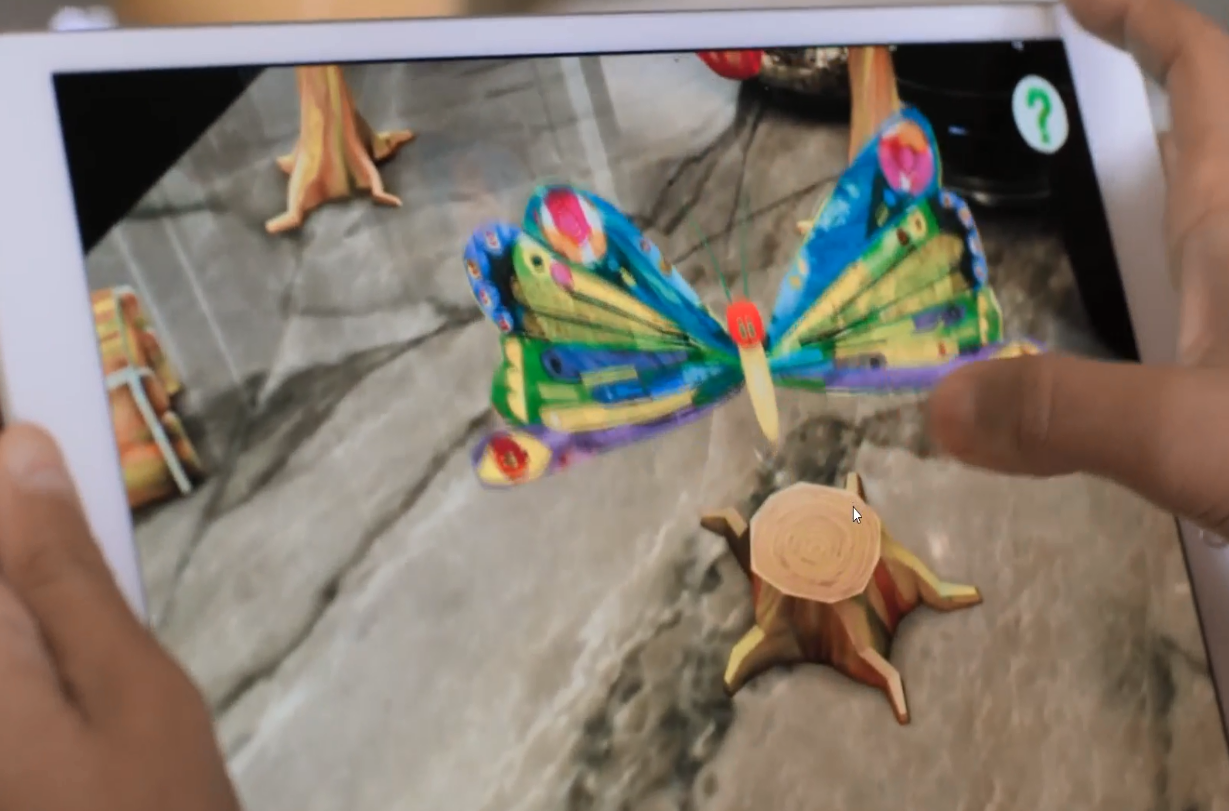
\includegraphics[width=\textwidth]{Img/1-ARExample.png}
    \bicaption{AR用于儿童教育行业。}{AR application for children education.}
    \label{fig:ARExample}
\end{figure}

\begin{figure}[!htbp]
    \centering
    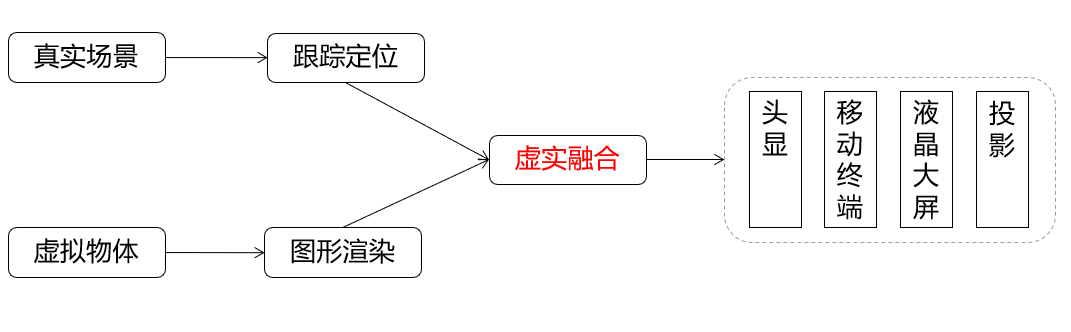
\includegraphics[width=\textwidth]{Img/1-ARflow.png}
    \bicaption{AR系统工作流程图。}{Work flow of AR system.}
    \label{fig:ARflow}
\end{figure}

增强现实系统的工作流程如图~\ref{fig:ARflow}所示。系统根据机器视觉技术在对相机跟踪定位,得到相机在真实场景中的位姿,通过虚实融合技术,
把通过计算机图形学技术渲染得到虚拟信息注册到真实场景中的恰当位置,将虚拟信息与真实场景相结合的结果呈现在头显、液晶屏等终端上,
提供虚实结合的交互效果。

能否精准地通过跟踪注册,将虚拟物体放置在真实场景中,很大程度上影响了增强现实系统能否给予虚拟图形准确的空间定位、物理遮挡、
透视形变、光照阴影等效果,进而决定着系统呈现的真实感和交互体验,这其中关键技术便是虚实融合技术。虚实融合技术是感知环境信息,
将渲染生成的虚拟信息与现实场景精准匹配、叠加的技术。具体来说,虚实融合技术可以从以下几个方面影响增强现实系统的真实感:

{
\setlist[enumerate]{}% restore default behavior
\begin{enumerate}[nosep]
    \item 时间一致性\\基于时间一致性的虚实融合主要关注增强现实系统的实时交互能力,确保虚拟物体与真实物体的运动关系相互协调,
    在时间序列上消除偏差,使得增强现实应用流畅、平滑、无延迟。
    \item 几何一致性\\基于几何一致性的虚实融合主要关注遮挡问题与物理约束,将虚拟信息在真实场景中精准定位。解决虚实遮挡问题
    依赖于对场景三维结构的了解,需要判断真实场景中的物体距离相机的距离,以及被遮挡部分的空间结构信息。物理约束方面,
    主要是约束虚拟物体与真实场景物体不重叠,保证虚拟物体的刚体结构及物理形变。
    \item 光照一致性\\基于光照一致性的虚实融合是根据虚实位置关系,渲染真实性强的光影关系,给虚拟物体添加与真实环境相适应的明暗、阴影等光照效果。
\end{enumerate}
}

我的研究主要集中于几何一致性的虚实融合方面,其关键是相机的跟踪注册技术。跟踪注册技术分为两方面,跟踪即估计相机在场景中的位姿,
得到每个时刻相机于三维场景中的相对位置和朝向。注册即获取场景的三维结构信息,同时将虚拟图形准确注册至真实环境,根据维场景空间
结构信息,准确在目标位置叠加虚拟图像。
\begin{figure}[!htbp]
    \centering
    \begin{subfigure}[b]{0.45\textwidth}
      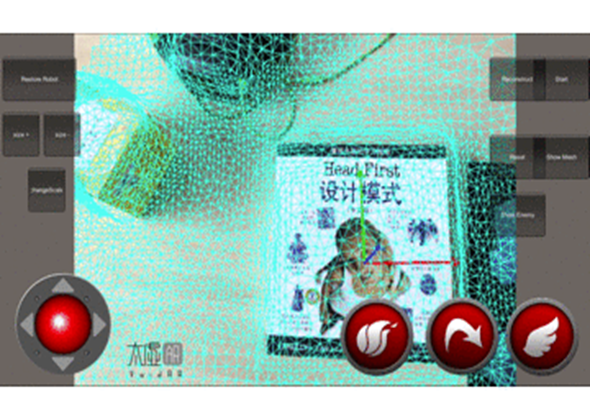
\includegraphics[width=\textwidth]{Img/1-senceUnderstand.jpg}
      \caption{}
      \label{fig:senceUnderstand}
    \end{subfigure}%
    ~% add desired spacing
    \begin{subfigure}[b]{0.45\textwidth}
      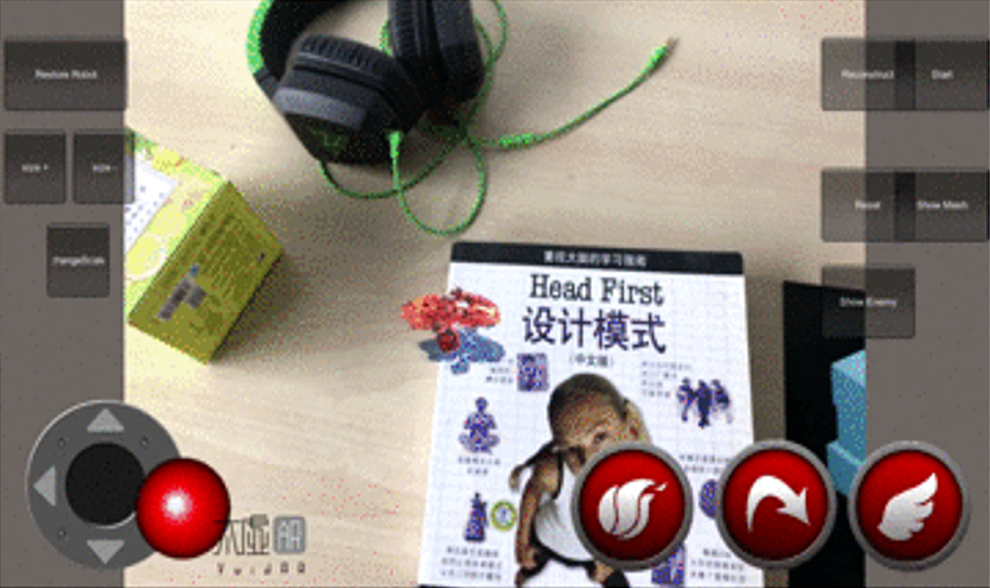
\includegraphics[width=\textwidth]{Img/1-senceUnderstandAR.png}
      \caption{}
      \label{fig:senceUnderstandAR}
    \end{subfigure}
    \bicaption{基于场景理解的AR系统。(a) 场景理解,(b) 虚拟物体跟踪注册。}{AR system based on scene understanding. (a) Scene understanding, (b) Virtual object registration.}
    \label{fig:scene}
\end{figure}

近年来,随着SLAM技术的高速发展,基于场景理解的跟踪注册技术逐渐成为一种新兴解决方案,图\ref{fig:scene}展示了一个基于场景理解的增强现实系统。SLAM(Simultaneous localization and mapping)技术全称即时定位与地图
构建,其目标是在未知环境下,通过相机、激光、惯性单元等传感器不断捕捉环境信息,实时的同步进行相机自身位姿的估计和未知环境的
三维地图构建。其中,以摄像机为数据获取源,基于特征匹配的视觉SLAM(Visual SLAM,V-SLAM)因其硬件需求较低,便携性更高,
在增强现实领域拥有更多应用空间。通过视觉SLAM技术,能够在未知场景下,无需提前布置或录入标志信息,同步获取高精度的跟踪定位结果和
三维环境感知结果,从而提供增强现实系统对于环境在三维层面的理解能力,从而提高跟踪注册精度。

然而,基于特征匹配的传统视觉SLAM技术仍存在一些问题:
{
\setlist[enumerate]{}% restore default behavior
\begin{enumerate}[nosep]
    \item 语义信息利用不充分\\传统SLAM系统并没有完全利用图像所蕴含信息,如高层的语义分割,物体级的目标检测等信息,仅提取了二维图像的局部特征。
    在位姿估计过程中,局部特征匹配提供的约束不够充分,所建地图仅能描述三维空间的几何结构,没有提供语义层面的表达。
    \item 难以应对动态场景\\在动态环境下,因基于视觉匹配的算法和硬件的限制,大多数传统视觉SLAM系统难以处理剧烈变化的动态环境,例如移动的人或物体,很容易
    大幅度影响相机位姿估计的表现,甚至诱发系统崩溃。同时在建图方面,传统视觉SLAM系统大多面向静态环境增量式建图,对于运动的物体
    易出现目标重影、模糊等问题。
\end{enumerate}
}

随着深度学习技术的发展,高层语义信息可以方便地通过卷积神经网络(Convolutional Neural Network,CNN)得到。通过
卷积神经网络,可以基于海量数据训练模型,完成目标检测、语义分割等任务,检测目标图像中的物体,输出其类别与位置,将每个
二维像素点赋予类别标签,给予其可解释的类别。

近年来,一些相关工作将深度网络与视觉SLAM框架相结合,能够识别环境中的独立个体,在传统视觉SLAM框架所建立的三维地图的基础上,
关联语义信息与几何信息,以此丰富三维地图的信息表达,建立具有语义信息和空间结构信息的场景地图,提高感知等级。同时能够在相机位姿估计过程中,根据语义信息提供更丰富的约束,
得到更精准的相机跟踪定位结果,并增强系统在动态环境下的鲁棒性。此类方法可称作语义SLAM(Semantic SLAM),它不但能够帮助系统
解决“目标在哪”的问题,还能够进一步明确“目标是什么”,是当前研究的热点和难点。

因此,语义SLAM技术能够帮助传统视觉SLAM框架提升位姿估计精度、动态场景下的鲁棒性和地图信息表达能力,进而能够帮助增强现实
系统在静态或动态场景下准确理解环境,计算得出虚拟信息在场景中应叠加投放的准确位置,提升跟踪注册的精度,用于优化增强现实系统中的虚实融合问题,
提高增强现实应用的真实感。因此,以上所述的传统视觉SLAM系统存在的问题,也是增强现实系统中基于场景理解的跟踪注册技术所面临的难点问题。
对于语义SLAM进行的研究,在增强现实领域具有一定的现实意义和应用价值。    

\section{国内外研究现状}\label{sec:ResearchStatus}
近年来,随着视觉SLAM系统的不断发展完善,其对于语义信息的利用也经历了从低层至高层的发展。以最初的低层局部特征为基础,发展出了
结构化的特恒工程,而后又开展了结合高层语义信息的语义映射和动态环境下的SLAM的研究。在增强现实领域中,语义SLAM相关研究更注重于
对环境的高层理解与表示,以及在动态环境下系统鲁棒性的和相机位姿估计精度的提升。
\subsection{传统SLAM框架}
传统SLAM框架大多包含负责跟踪的前端和负责优化的后端两大主要模块,其中前端模块按照特征提取方法可分为特征点法和直接法两类,后端模块
又可根据优化方法分为基于滤波的方法和基于非线性优化的方法两类。早期SLAM框架大多包含基于特征点法的前端模块和基于滤波方法的后端模块。
Andrew J Davison等人于2007年提出的MonoSLAM是基于特征点的SLAM的先驱之作,它通过扩展卡尔曼滤波
(Extended Kalman Filter,EKF)进行后端优化,保证了单目SLAM的实时性,但只能应用于较小的场景。随后,Klein 与 Murray 等人开创性地采用基于非
线性优化的方法以克服滤波技术的局限,提出了PTAM\citep{Klein2007Parallel}系统,将跟踪与建图作为两个分开的线程,获得更加稠密与更大范围的场景结构,
无论在精度还是鲁棒性等方面都取得了比基于滤波的方法更好的表现,但在处理的场景规模和稳定性方面仍有提升空间。

PTAM的思想奠定了SLAM领域研究的方向和基础,在此之后,众多研究机构提出了很多当前性能优秀的SLAM框架。西班牙Zaragoza大学的Raúl Mur-Arta
等人于2015年提出的ORB-SLAM\citep{mur2015orb}首次将地图初始化、视觉里程计、后端优化、闭环检测等模块集成至一个完整系统,其主要思想是
对相机捕获的图像提取ORB\citep{Rublee2012ORB}特征并在连续帧间进行特征匹配,构造重投影误差并以非线性优化的方法进行优化。
而后其在2017年又提出了ORB-SLAM2\citep{mur2017orb},更进一步加入了重定位模块,成为现今最为完整、高效的基于特征点的稀疏SLAM系统之一。
与之不同,Jakob Engel等人在2014年提出了基于直接法的LSD-SLAM\citep{Engel2014LSD},此方法无需图像特征提取与匹配,而是基于像素间的光度误差直接优化,
并进行半稠密的重建。随着RGB-D相机的发展,基于深度数据的SLAM系统亦开始涌现。帝国理工大学的Thomas Whelan等人在2015年提出了
ElasticFusion\citep{whelan2015elasticfusion},此方法采用几何误差和光度误差联合优化,使用面元结构建模,在不断优化迭代中
提高位姿估计和地图构建精度。

然而,这些方法都仅通过低层的局部特征匹配或像素匹配来构造约束、进行优化,所建地图也仅限于几何层面,没有结合高层语义信息。此外,
这些方法都面向静态环境,在动态场景下,其相机位姿的估计精度将受到很大影响。

\subsection{语义映射}
传统SLAM构造的三维地图仅包含几何信息,难以满足复杂的任务需求。语义映射能够将二维语义信息与三维几何地图相关联,逐渐成为了一个
热门的研究领域。这类工作通过深度网络或几何方法对二维图像帧进行语义分割,获取像素级的语义标签,再通过特定规则与三维路标点关联匹配,
以构造同时含有语义信息和几何信息的三维地图。

同样来着帝国理工大学的工作SemanticFusion\citep{MccormacSemanticFusion}以它使用ElasticFusion为基础,使用FCN\citep{long2015fully}进行
语义分割,同时使用条件随机场(Conditional Random Field,CRF)优化分割结果,语义匹配方面,使用贝叶斯更新方法将二维语义与三维地图进行数据关联,
系统除构建了语义地图外,还验证了SLAM系统所捕获的连续帧能够辅助优化二维语义分割结果。
来自东南大学的Li X等人\citep{LiSemi}使用深度网络模型DeepLab-v2\citep{Chen2014Semantic}进行二维图像的语义分割,该网络结构包含
孔洞卷积和空间池化金字塔(ASPP),辅以条件随机场进行地图正则化,能够平滑语义分割结果中的噪声。此方法同样使用贝叶斯更新方法
进行数据关联,结合LSD-SLAM,解决了室内、室外不同场景下的尺度问题,其构建的语义地图也有一定精度提升。来自国防科技大学的Qi等人\citep{qi2018deep}
使用点云建图,并关联语义标签,并通过图分割方法将点云分为聚类的超体,迭代获取更精细的平面部分,优化了语义建图的细节。
除此之外,Hoang等人\citep{hoang2019high},Zeng等人\citep{zeng2018semantic}以及CNN-SLAM\citep{tateno2017cnn}等工作都从不同
角度提升了语义关联或语义建图的精度。

这些方法使用的语义信息为像素级别,对于优化相机位姿估计或辅助增强现实应用开发的提升价值有限。在此之上,实例级的语义分割信息
同时包含物体级的目标检测结果和像素级的语义分割结果,有着更高的研究价值和应用潜力。N. Sunderhauf等人\citep{S2017Meaningful}
使用物体识别框架SSD\citep{Liu2016SSD}进行目标检测,对关键帧图像生成固定数量的物体框,并给出目标分类结果和置信度。
语义分割部分则选择了使用基于超体元的分割点云模型,通过最近邻方法将目标检测结果映射到分割后的点云模型上,得到具有物体级标签的语义地图。
Fusion++\citep{mccormac2018fusion++}使用稠密SLAM系统KinectFusion\citep{Newcombe2011KinectFusion}中的三维重建方法,
结合同步进行目标检测、语义分割的深度网络Mask R-CNN\citep{HeMask},将二维图像检测到的物体以TSDF(Truncated Signed Distance Function)
方法增量式建立三维模型,得到物体级的语义地图。

然而以上方法仅单纯地将二维语义信息与三维几何地图进行了关联映射,并未利用语义信息优化SLAM的核心任务之一——状态估计。此外,
这些工作仅面向静态环境开展,传统视觉SLAM在动态环境下面临的位姿估计不准、建图出现重影等问题,在这些系统中依旧存在。

\subsection{动态环境下的SLAM}
SLAM系统所面对的困难场景之一是动态环境,三维物体的运动和相机自身的抖动都可能为状态估计环节引入误差,也会使得所建的三维地图出现重影等问题。
现有的一些传统视觉SLAM算法在这方面还很比较薄弱,而一些近期的工作开始尝试利用语义信息来解决这些问题。

2018年帝国理工大学提出的MaskFusion\citep{runz2018maskfusion}也使用Mask R-CNN进行实例分割,同时针对网络分割结果的边缘不精确
问题,使用了几何方法在二维图像上进行细化边缘,与深度网络的分割结果相结合,得到物体级的语义标签。此方法能够对前景物体单独建模、
跟踪和维护,实现了动态场景下的物体级建图,但MaskFusion并未解决动态环境对位姿估计带来的误差问题。
来自清华大学的Yu等人提出了DS-SLAM\citep{YuDS},利用SegNet\citep{VijaySegNet}实时获取像素级的语义标签,结合基于光流的运动一致性
检测方法来滤除场景中如行走的人等的动态部分的特征点,依次减少动态目标对于位姿估计的影响。然而此方法仅使用了像素级的语义分割结果,
没有进行物体级建图,此外,仅滤除了属于“人”这一个类别的动态目标的特征点,没有考虑不同类别物体的影响。
Berta等人于2018年发表的DynaSLAM\citep{BertaDynaSLAM}能够通过多视图几何、深度学习或二者结合的方法检测场景中的运动物体,
并将属于运动目标范围内的特征点移除,从而提高位姿估计精度。但这种方法粗暴地移除了属于某一语义类别的全部特征点,容易因剩余特征点
数量过少而导致跟踪失败,而与DS-SLAM相似,DynaSLAM没有考虑不同类别物体的影响,也没有建立动态环境下的物体级语义地图。

这些方法都为克服传统视觉SLAM在动态场景下的局限,结合语义信息做出了一些努力,取得了相应成果。但它们没有完全利用语义信息,
同时优化位姿估计和建立物体级语义地图,在这一方面仍有很大的研究空间,需要后续的大量实验和探索。

\section{论文主要研究内容}
基于目前所积累的理论知识、研究思路和实验数据,本文对基于语义SLAM,对动态场景下位姿估计优化方法、语义地图的构建和表示方法及
在增强现实系统中的应用方法进行了研究,力图以基于语义信息的SLAM改进方法为核心技术,提高增强现实系统的虚实融合性能,
提升系统的真实感体验,解决一系列涉及到的问题。
\begin{figure}[!htbp]
    \centering
    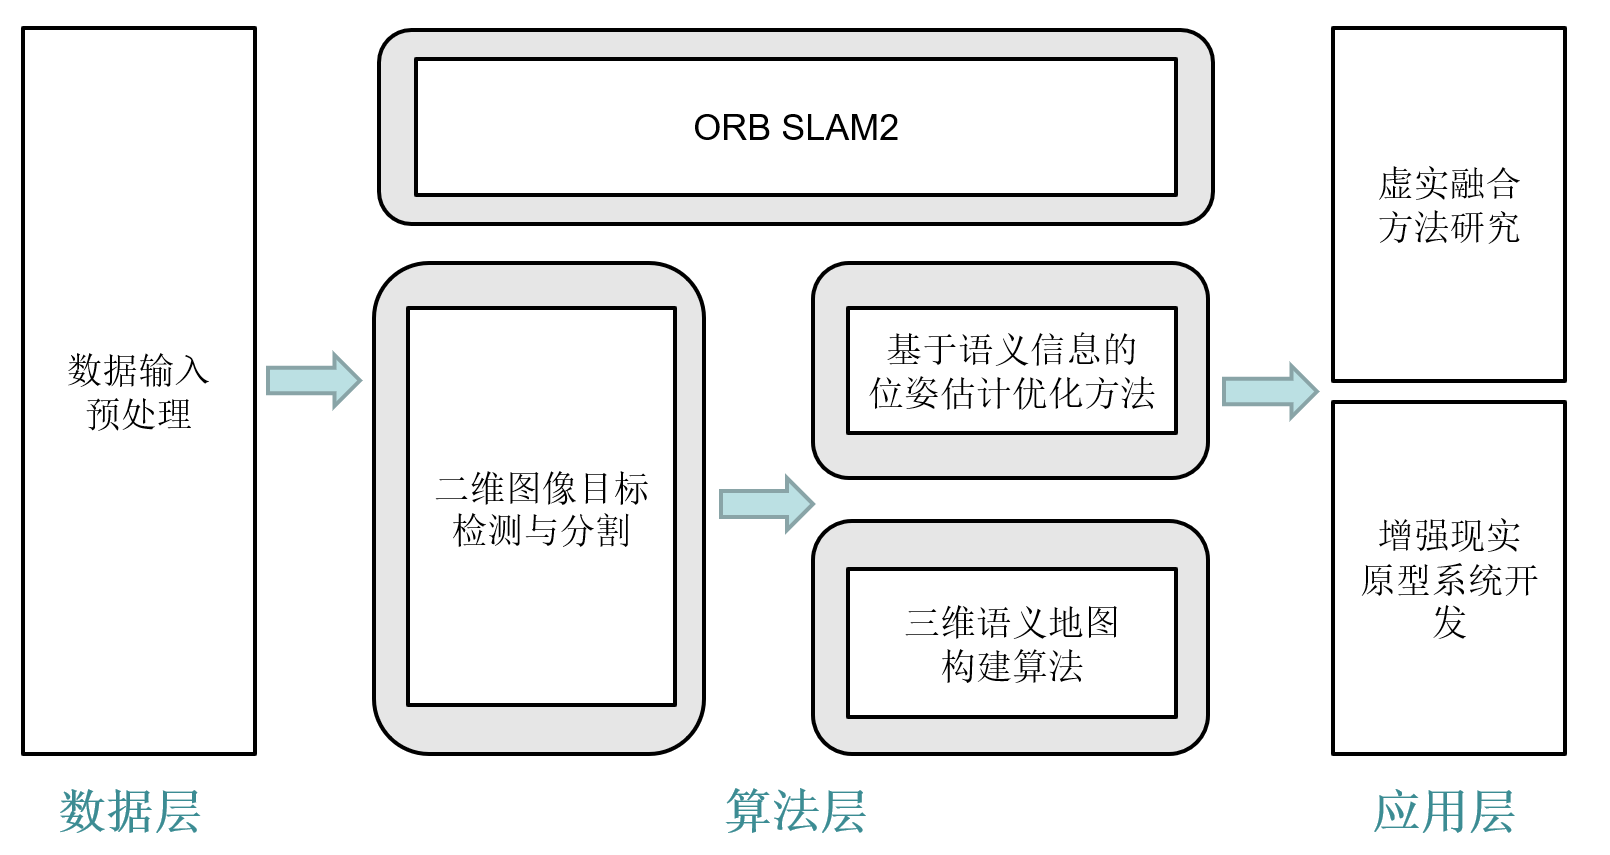
\includegraphics[width=\textwidth]{Img/1-researchFramework.png}
    \bicaption{系统研究框架。}{Research framework of this paper.}
    \label{fig:researchFramework}
\end{figure}
本文工作主要体现在以下几个方面:
{
\setlist[enumerate]{}% restore default behavior
\begin{enumerate}[nosep]
    \item 动态场景下基于语义信息的位姿估计优化方法\\这部分研究工作针对动态场景,提出了双阶段的动态外点滤除算法,此算法结合基于语义类别的
    自适应权重生成方法和基于极线约束的动态一致性检测方法,能够对于不同类别的物体自适应生成不同的判定条件,判断其是否处于运动状态,
    并移除处于运动状态的物体的轮廓内的特征点。此算法在TUM RGB-D数据集上进行了验证,在动态场景下其结果比ORB-SLAM2有数量级式的提升,
    提升幅度在大部分指标上优于业界先进系统,表明它能够有效减少环境中运动物体对于SLAM系统位姿估计的干扰,提升基于特征的视觉SLAM系统在动态场景下的位姿估计精度和鲁棒性。
    \item 语义地图的构建和表示方法\\这部分研究工作针对不同层级语义地图对环境的表示能力,分别探究了基于局部特征的预置语义库地图和语义SLAM系统生成的
    物体级三维语义点云地图的构建和表示方法。对于预置语义库地图提出了特征识别和跟踪方法,验证了其对室外环境的表示能力和在增强现实导航系统中的应用能力。
    对于物体级三维语义点云地图,本文提出了针对语义类别的物体跟踪策略,能够对环境中的物体分别建模、跟踪,适应动态变化的环境,并进行语义关联。
    此方法在动态环境和静态环境下分别进行了验证,结果表明它能够提高建图的鲁棒性,建立随环境变化而变化的物体级语义地图,从而提高对三维环境的表示能力。
    \item 增强现实原型系统的设计与实现\\这部分研究工作设计并实现了一个增强现实原型系统,融合了述研究的算法,在虚实融合阶段进行了
    优化,提升了系统的真实感体验。
\end{enumerate}
}

\section{论文组织结构}
第一章介绍了本文研究的背景和意义,详细列举了国内外相关研究现状,明确了本文的研究工作并给出了本文的章节安排。

第二章从整体上介绍了本文所提出系统的框架结构,包括所用的视觉SLAM框架、深度神经网络以及本文所设计的结合二者的语义SLAM框架。

第三章详细描述了本文所研究的动态场景下基于语义信息的位姿估计优化方法,给出了此算法在公开数据集的测试数据,与当前主流视觉SLAM框架和
先进同类方法进行了对比分析。

第四章聚焦语义地图的构建和表示方法,分别叙述了基于局部特征的预置语义库地图和物体级三维语义点云地图的构建和表示,并
对其效果分别进行了评估。

第五章介绍了本文基于算法理论研究,设计并实现的增强现实原型系统,给出了其在虚实融合方面的性能和真实感体验的测试与分析。

第六章对于本文所述的全部工作进行了整体总结,分析了当前存在的不足和提升空间,列出了后续应开展的工作内容,对未来研究前景进行了展望。

\chapter{系统框架介绍}\label{chap:framework}
\section{引言}
本文的研究采用基于特征的视觉SLAM框架ORB-SLAM2作为基础SLAM解决方案,以提供位姿估计和几何建图功能。同时,结合了实例级的语义
分割网络Mask R-CNN,对输入的彩色图像进行预测,同步得到目标检测和像素级语义分割结果。在语义建图方面,采用了PCL点云库\citep{rusu20113d}
进行物体级的三维点云地图的构建。本章将介绍本文所研究系统的各基础部分的原理与及结构,并给出系统的整体框架描述。
\section{基于特征的视觉SLAM框架}
\subsection{视觉SLAM综述}
基于特征的视觉SLAM通过视觉传感器获取的数据流,表示为$\mathbb{F}=\left\{F_{0},...,F_{k},...,F_{N}\right\}$,
在时刻$k$,$F_{k}$表示第$k$帧的输入,可能包括彩色图$C_{k}$和深度图$D_{k}$。SLAM系统的基本任务是
估计相机的位姿和路标点集合,相机位姿为每个时刻相机自身相对于世界坐标系的转移矩阵,可表示为$\mathbb{T}=\left\{T_{0},...,T_{k},...,T_{N} \right\}$,
其中,$T_{k}$表示第$k$帧相机位姿,记为:
$$T_{k}=
\begin{gathered}
\begin{bmatrix} R_{k} & t_{k} \\ 0 & 1 \end{bmatrix}
\end{gathered}
$$
$R_{k}\in SO\left(3\right)$,表示此帧的旋转矩阵,$t_{k}\in \mathbb{R}^{3x1}$,表示此帧的平移向量。实际运算过程中,SLAM系统常常
先推算得出相邻帧$F_{k-1}$与$F_{k}$之间的转移矩阵,表示为:
$$T_{k-1,k}=
\begin{gathered}
\begin{bmatrix} R_{k-1,k} & t_{k-1,k} \\ 0 & 1 \end{bmatrix}
\end{gathered}
$$
其中$R_{k-1,k}\in SO\left(3\right)$,表示相邻阵间的旋转矩阵,$t_{k-1,k}\in \mathbb{R}^{3x1}$,表示相邻帧间的平移向量。
第$K$帧的位姿转移矩阵可以由$k-1$的位姿和两帧间的转移矩阵计算得出:
$$T_{k}=T_{k-1,k}T_{k-1}$$,而初始帧的位姿$T_{0}$常常由用户初始化为世界坐标系原点。

SLAM系统的另一项任务是估计路标点在世界坐标系中的坐标,路标点的集合可以表示为$\mathbb{L}=L_{0},...,L_{k},...,L_{M}$,
其中第$k$个路标点可以表示为$L_{k}=(x_{k},y_{k},z_{k})$。

一个完整的视觉SLAM系统可以在未知场景中同步解决以上两个问题,如图\ref{fig:SLAMflow}所示,其框架一般来说主要包括传感器数据读取、视觉里程计、后端优化、回环检测、
地图构建五个部分。具体流程为,首先由视觉传感器获取对于场景的观测信息,由视觉里程计模块负责进行帧间特征提取与匹配,完成对于相机位姿和路标点在全局坐标系下的初步估计,
得到相机轨迹和三维路标点坐标。后端模块会对系统的状态变量进行优化,得到全局最优的估计值。同时,同步运行回环检测模块,
以解决前端模块中出现的累积漂移误差。最终通过地图构建模块,生成可视化的三维地图。下面将逐模块详细介绍其工作原理。
\begin{figure}[!htbp]
    \centering
    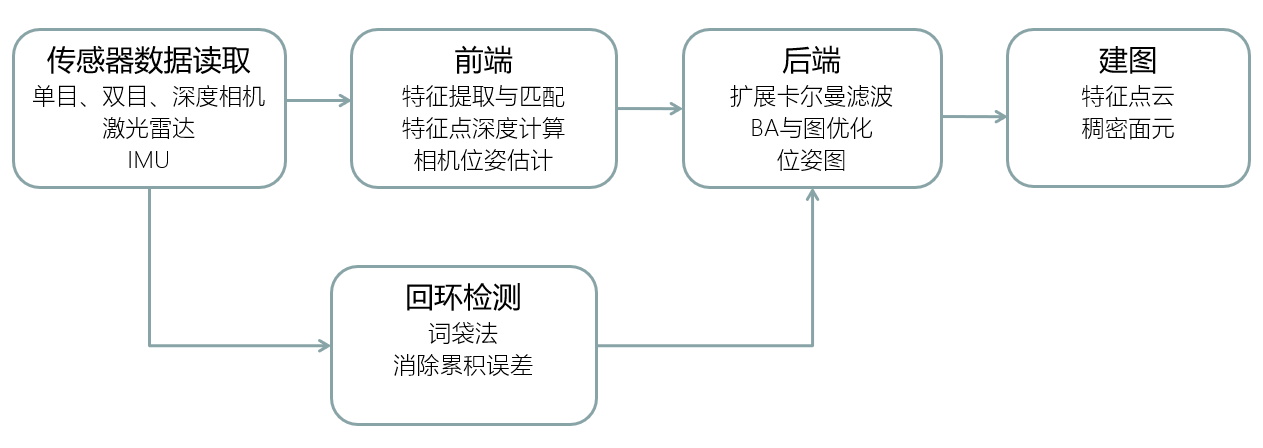
\includegraphics[width=\textwidth]{Img/2-SLAMflow.png}
    \bicaption{典型SLAM系统结构。}{Typical SLAM system architecture.}
    \label{fig:SLAMflow}
\end{figure}
\subsubsection{传感器数据读取}
视觉SLAM系统仅通过相机作为传感器来捕捉环境信息,它随着设备的移动,以恒定帧率进行拍摄,形成视频流作为系统输入。根据相机工作方式,
所用相机可以分为单目相机、双目相机、RGB-D相机三种。

其中单目相机仅有一个摄像头,其工作原理比较简单,但若想通过单目相机的数据恢复场景三维结构,必须通过移动过程中拍摄的连续帧图像,
根据视角变换造成的视差变化推测真实物体的相对距离。但单目相机仍存在尺度不确定性,通过单目相机观测数据估计的相机轨迹和三维地图
都将与真实值相差一个尺度因子。

与单目相机相比,双目相机增设了一个摄像头,通过两个摄像头同时进行拍摄,形成了天然的视差,两个摄像机之间的距离称作基线(Baseline),
通过已知的基线,可以恢复场景三维场景,消除尺度不确定性。但双目相机于单目相机都存在一个问题,即在计算路标点三维坐标时,
依赖于三角化算法以获取深度,需要大量的计算资源。

RGB-D相机使用了不同的深度值获取算法。它主要依靠相机的物理原件,如红外摄像头,激光发射器等,通过结构光或ToF(Time-of-Flight)
技术直接测量出场景中物体距离相机的距离。通过物理测量方法,可以节省大量的计算资源,但目前大多数RGB-D相机仍存在对光照变化敏感、
测量范围小等问题,因此更多用于室内场景。

\subsubsection{视觉里程计}
视觉里程计又称作前端模块,它的任务是估计相邻帧之间描述相机运动的转移矩阵和当前帧可见的路标点的三维坐标,以形成相机位姿轨迹
并构造局部地图。对于基于特征的视觉SLAM系统来说,前端模块的实现主要基于特征点法,它的思路是从每帧图像中提取能够描述局部特征的特征点,
这些特征点在相机视角发生变化后能够保持稳定,可以计算出匹配的特征点集。在传统图像处理领域,研究者们提出了多种方法来描述图像
局部特征,如SIFT\citep{LoweDistinctive}、SURF\citep{Bay2006SURF}、ORB\citep{Rublee2012ORB}等。目前由于计算资源的限制,
提取并匹配SIFT和SURF特征点无法满足SLAM系统的实时性需求,而ORB特征点成为了一个可用的选择。
ORB(Oriented FAST and Rotated BRIEF)特征是一种具有旋转不变性和尺度不变性的快速特征提取和描述方法,它分为负责特征提取的oFast
和负责特征描述的rBRIEF两部分。oFAST由FAST关键点改进得到,FAST的核心思想是以与邻域内灰度相差较大的点为关键点,oFAST在此基础上
引入了尺度金字塔,计算不同尺度上的FAST关键点。同时,oFAST还使用矩描述FAST关键点的方向,为其引入了旋转不变性。对于一FAST关键点$P(x,y)$,矩$m$的定义为:
$$m_{pq}=\sum_{x,y \in r} x^{p}y^{q}I(x,y)$$
其中$I(x,y)为$该点灰度值。该关键点的方向角$\theta$为:
$$\theta =arctan\left(\frac{m_{01}}{m_{00}}/\frac{m_{10}}{m_{00}}=arctan(\frac{m_{01}}{m_{10}})\right)$$

rBRIEF则由BRIEF描述子演化而来,BRIEF对关键点周围一定数目的点对进行灰度值比较,根据其大小关系生成二进制串作为描述符,具有匹配
速度快的特点。rBRIEF在此基础上,以关键点和取点区域的形心连线来建立二维坐标系,以此增加了旋转一致性。

在视觉SLAM视觉里程计模块中,完成特征点提取及匹配后,可选择而不同算法求解相邻阵间的转移矩阵:

\emph{\textbf{2D-2D}}\\
    若连续两帧仅有2D图像上的特征点描述,则通过对极几何关系求解本质矩阵或基础矩阵,以恢复相机运动矩阵。相邻两帧之间的运动关系
    可以通过本质矩阵(Essential Matrix)描述,表示为$E$,其包含了相机的旋转和平移变换参数,以及一个未知的平移变换因子,可以表示为:
    $$E\simeq t^{X}R$$
    其中$\simeq$表示等式两侧相差一个尺度因子。$t=\left[t_{x},t_{y},t_{z}\right]$,为平移向量,而
    $$
    t^[X]=
    \begin{gathered}
    \begin{bmatrix} 0 & -t_{z} & t_{y} \\ t_{z} & 0 & -t_{x} \\ -t_{y} & t_{x} & 0 \end{bmatrix}
    \end{gathered}
    $$
    表示平移变换,而$R$为其旋转矩阵。
    对于$F_{k-1}$和$F_{k}$上在相机坐标系下匹配的两点$X_{k-1}^{i}=\left[x_{k-1}^{i},y_{k-1}^{i},z_{k-1}^{i}\right]$和$X_{k}^{i}=\left[x_{k}^{i},y_{k}^{i},z_{k}^{i}\right]$,根据极线约束可以得出:
    $${X_{k-1}^{i}}^{T}EX_{k}^{i}=0$$
    而对于在像素平面上的两匹配二维点$P_{k-1}=\left[u_{k-1}^{i},v_{k-1}^{i} \right]$和$P_{k}^{i}=\left[u_{k}^{i},v_{k}^{i}\right]$,可得它们的齐次坐标${\widetilde P_{k-1}^{i}}=\left[u_{k-1}^{i},v_{k-1}^{i},1 \right]$和${\widetilde P_{k}^{i}}=\left[u_{k}^{i},v_{k}^{i},1 \right]$。
    通过内参矩阵$K$,可以进行像素平面上齐次坐标与相机坐标系下点的转换:
    $$
    Z{\widetilde P}
    =
    Z
    \begin{gathered}
    \begin{bmatrix} u \\ v \\ 1 \end{bmatrix}
    \end{gathered}
    =
    \begin{gathered}
    \begin{bmatrix} f_{x} & 0 & c_{x} \\ 0 & f_{y} & c_{y} \\ 0 & 0 & 1 \end{bmatrix}
    \end{gathered}
    \begin{gathered}
    \begin{bmatrix} X \\ Y \\ Z \end{bmatrix}
    \end{gathered}
    =
    KX
    $$
    其中$f_{x}$、$f_{y}$为相机焦距,$c_{x}$、$c_{y}$为主点平移。
    
    相似地,对于像素平面上的匹配点,可以由基础矩阵(Fundamental Matrix)$F$表示两帧间的极线约束关系:
    $${\widetilde{P_{k}^{i}}}^{T}F{\widetilde{P_{k-1}^{i}}}^{T}={\widetilde{P_{k}^{i}}}^{T}EK^{-1}{\widetilde{P_{k-1}^{i}}}^{T}=0$$

    $E$或$F$可以通过八点法(Eight-point-algorithm)\citep{HartleyIn},\citep{LONGUET1981A}以匹配点对组构造线性方程组解出,
    进而可以通过奇异值分解(SVD)得到相机的运动$R,t$。
    
\emph{\textbf{2D-3D}}\\若连续两帧图像中有一帧特征点对应的3D空间位置已知,则可以通过PnP(Perspective-n-Point)算法估计相机运动。
它最少仅需要3对匹配点,就能构造出线性方程组,进而解出相机转移矩阵,PnP问题的解法包括P3P\citep{GaoComplete}、EPnP\citep{lepetit2009epnp}、直接线性变换(DLT)等。
此外,也可以构造重投影误差:
$$T_{k-1,k}^{*}=\mathop{argmin}\limits_{T_{k-1,k}}\frac{1}{2}\sum\limits_{i=1}^{n}\left \| P_{k-1}^{i}-\pi \left(KT_{k-1,k}X_{k}^{i}\right) \right \|^{2}$$
其中$\pi$是将相机坐标系下的点变换至像素平面上的点的变换。通过非线性优化的方法,可以最小化重投影误差,求得最优的变换矩阵。

\emph{\textbf{3D-3D}}\\若连续两帧图像特征点对应的3D空间位置都已知,则可以通过迭代最近点(Iterative Closest Point, ICP)算法对这两组具有匹配关系的三维点进行运动估计。
一般来说,ICP问题也通过非线性优化方法求解,其构造的误差为:
$$T_{k-1,k}^{*}=\mathop{argmin}\limits_{T_{k-1,k}}\frac{1}{2}\sum\limits_{i=1}^{n}\left \| \widetilde{X}_{k-1}^{i}-T_{k-1,k}\widetilde{X}_{k}^{i} \right \|^{2}$$
其中$\widetilde{X}$表示在相机坐标系下一点$X$的齐次坐标。

计算特征点对应的路标点,即其在世界坐标系下的三维坐标,可以通过三角化(Triangularization)方法,其思想是对于同一三维点在两帧
上的投影$P_{k-1}^{i}$和$P_{k}^{i}$,它们与各自相机光心所连成的直线会在三维空间中交于一点。根据这一关系,可以构造等式,通过
最小二乘法求解得到三维点的深度值。此外,若相机能够捕捉得到深度图像,则可以方便地从深度图像中获取三维点坐标,避免了三角化过程
的计算开销。

基于特征匹配的相机位姿求解方法成为特征点法,它对于系统运行时的光照、旋转和尺度变化比较鲁棒,是长久以来比较成熟的解决方案,已具
有广泛应用。然而特征点的提取和匹配环节仍是当前SLAM系统最为耗时的一个部分,此外,在如白色墙壁等纹理缺失的场景下,提取的特征点数目会急剧下降,导致跟踪失败。

近年来学者们提出了直接法,可以能够一定程度上克服特征点法的缺点。直接法的思想是不提取图像中的特征点,而是根据相邻图像之间的灰度值
差异,构造并最小化光度误差(Photometric Error),直接恢复相机的运动。然而直接法也有一定的局限,即它的前提是灰度不变假设,因此在环境亮度变化剧烈的场景下,直接法会面临失效的风险。
$$T_{k-1,k}^{*}=\mathop{argmin}\limits_{T_{k-1,k}}\sum\limits_{i=1}^{n}\left \| I_{k-1}(P_{k-1}^{i})-I_{k}(P_{k}^{i}) \right \|^{2}$$
其中,$I(P)$为一像素平面上点$P$对应的灰度值。

\subsubsection{后端优化}
后端优化模块的主要目标是最小化SLAM过程中的因噪声等原因引入的误差,让状态估计在局部或全局下最优。其优化的目标变量是整个系统的状态变量,
即相机位姿$\mathbb{T}$和路标点集合$\mathbb{L}$。在后端优化过程中,系统的状态被抽象为一个概率模型,对于变量状态不确定性的估计
则看做一个最大后验概率估计(Maximum-a-Posteriori, MAP)过程。当前广泛应用的后端优化方法主要分为基于滤波器的优化方法与非线性优化方法。

基于滤波器的方法假设了系统的马尔科夫性,即当前时刻的状态仅与上一时刻相关。在线性高斯系统中,可以通过系统运动模型确定状态变量的先验分布,
并通过观测模型得到状态变量的似然分布,而后求解最大后验概率估计,同时也是线性系统的最优无偏估计,这一过程即为卡尔曼滤波(Kalman Filtering,KF)。
而SLAM系统中的运动模型和观测模型通常为非线性函数,因此可以以泰勒展开的方法将其近似为线性的高斯分布,以应用卡尔曼滤波算法,即扩展卡尔曼滤波(Extended Kalman Filtering,EKF)。

相比基于滤波器的方法,基于非线性优化的方法有更广泛的应用。这种方法的思想是根据全局或多帧之间变量的投影、变换、匹配等关系构造不同的约束,
使用非线性优化方法最小化误差,以得到最优的估计值。通常使用的约束包括三维点到二维平面投影所构成的约束和相机位姿的变换关系构成的约束:
$$\mathop{min}\limits_{T_{0},...,T_{N},L_{0},...,L_{M}}\sum\limits_{i=1}^{N}\sum\limits_{j=1}^{M}\left \| h(T_{i},L_{j})-l_{i,j} \right \|$$
$$\mathop{min}\limits_{T_{0},...,T_{N}}\sum\limits_{i=1}^{N}\sum\limits_{j=1}^{N}\left \| T_{i}-T_{i,j}T_{j} \right \|^{2}$$
其中,$h(T_{i},L_{j})$表示将三维路标点$L_{j}$通过第$i$帧的转移矩阵投影到二维平面$F_{i}$上的变换。

\subsubsection{回环检测}
由于前端模块仅考虑相邻帧之间的关联,每一帧位姿的估计都是建立在前一帧的估计结果之上,因此在程序运行过程中,前一帧产生的估测误差
将会不可避免的累积到下一帧上,随着程序运行时间增长,这一误差将逐渐变大,整个SLAM系统变出现了累积误差。针对这一问题,回环检测模块
的目标是在相机经过之前到达过的地方时,根据对同一地点不同时刻的观测建立约束,减少系统的累积误差,得到全局一致的状态估计。

回环检测模块的关键是如何高效地判断相机当前的观测是否曾出现过,词袋法(Bag-of-Words,BoG)是一种广泛应用的解决思路,它的核心是
用向量表示图像上的特征种类,以此描述一张图像,将两张图像向量间的距离则表示图像的相似程度。在实际应用中,如何高效比较这一向量的
相似性至关重要,利用数据结构分层存储和查找可以显著提高其效率,K-mens聚类和K叉树可以将算法复杂度降到对数级别,
是一种很好的选择,图\ref{fig:kdTree}展示了经典的KD树结构。
\begin{figure}[!htbp]
    \centering
    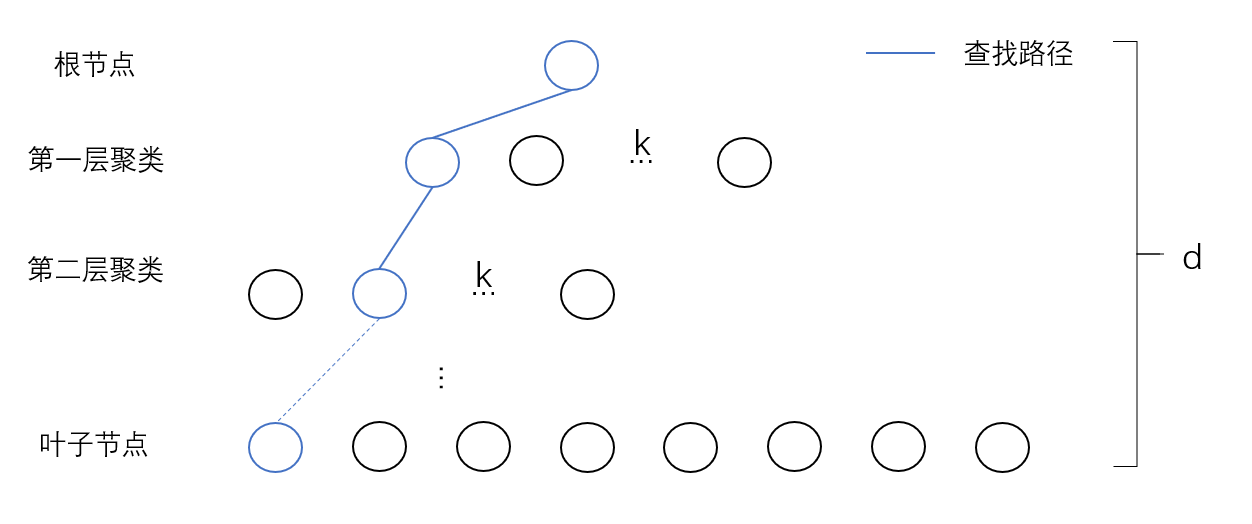
\includegraphics[width=\textwidth]{Img/2-kdTree.png}
    \bicaption{KD 树结构。}{KD tree architecture.}
    \label{fig:kdTree}
\end{figure}
\subsubsection{地图构建}
SLAM系统中地图构建模块的目标是根据已估计得到的相机位姿和路标点坐标,生成可视化的三维地图。传统SLAM生成的地图仅包含几何结构信息,
根据表示程度的不同,可以分为稠密地图和稀疏地图。建立稠密地图的方法包括TSDF建模、、面片(Surfel)模型、三角网格(mesh)建模、稠密点云、基于体素(Voxel)的八叉树模型等,
ElasticFusion是这一类别的代表工作,它融合RGB-D输入,以面片建立了室内场景地图模型。

对于基于特征的SLAM系统,更多建立的是稀疏地图,地图以路标点为单位。建立路标点首先需要在纹理丰富的关键帧中抽取特征点,经三角化或使用深度图
得到其深度信息,然后根据此关键帧的转移矩阵,将相机坐标系下的特征点变换到世界坐标系中,成为三维地图中一点。除此之外还需要
在后端优化模块对三维地图点集进行坐标优化,使其重投影误差最小化。整个地图构建模块与视觉里程计和后端优化模块环环相扣,是其对
环境感知结果的可视化表达。

\subsection{ORB-SLAM2结构简介}
ORB-SLAM2是当前最完善的基于特征的SLAM框架之一,在大多数场景下都有着出色的跟踪、建图表现和鲁棒性。本文的研究便以ORB-SLAM2为基础,
它能够接收受单目、双目、RGB-D格式的图像输入,包含位姿估计、稀疏建图、局部与全局优化、闭环检测与闭环纠正等功能,其系统分为跟踪(Tracking)、
局部地图(Local Mapping)、回环闭合(Loop Closing)三个线程,具体系统结构如图\ref{fig:orbslam}所示。
\begin{figure}[!htbp]
    \centering
    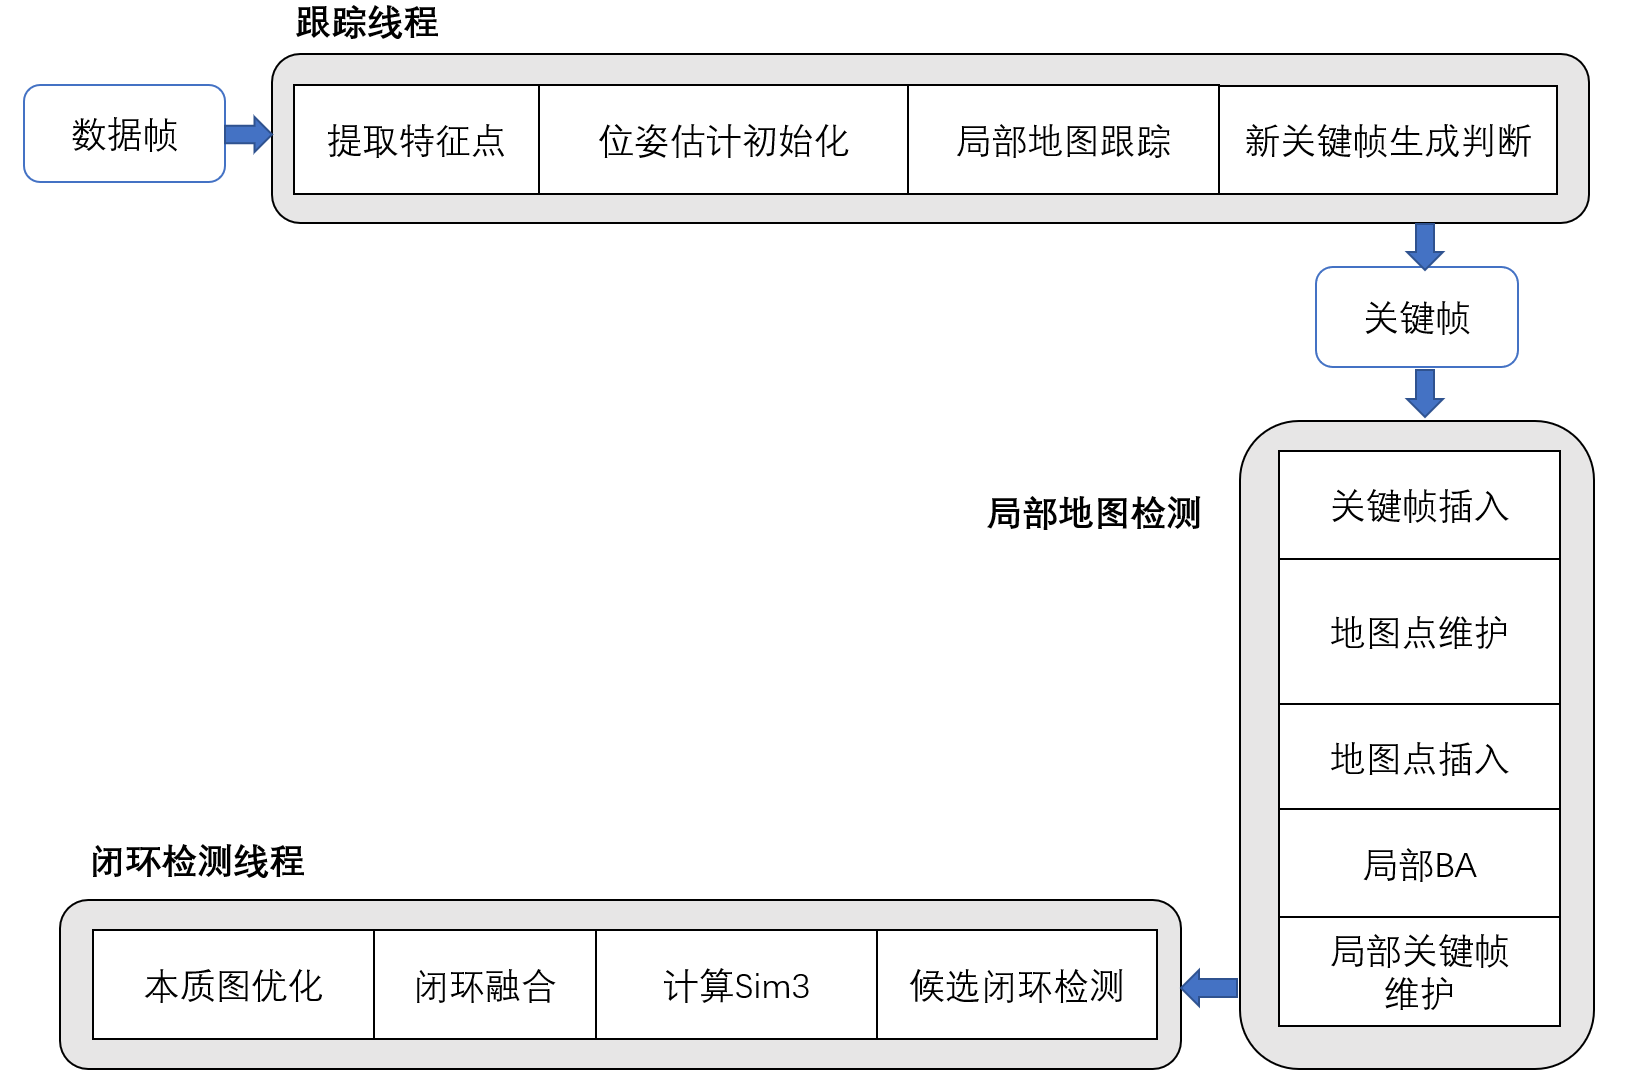
\includegraphics[width=\textwidth]{Img/2-ORBSLAM.png}
    \bicaption{ORB-SLAM2系统结构。}{System architecture of ORB-SLAM2.}
    \label{fig:orbslam}
\end{figure}
相机捕获的图像数据流首先输入跟踪线程,系统从中提取ORB特征点,在相机稳定移动的情况下根据相邻帧间特征点匹配结果,以恒速模型
初始化相机位姿的估测值,若相机运动较剧烈,也可通过参考帧或重定位的方法进行位姿初始化,这一操作也增加了系统的鲁棒性。同时,
对于单目或多目的数据输入,系统还会通过三角化算法得到特征点的深度值。之后,在当前帧的局部范围内将进行局部地图跟踪,轻量级地
进行优化。最后,在跟踪线程中还将判断并生成关键帧。

关键帧将输入局部地图线程,用于更新和维护路标点集合,并通过局部捆绑调整的方法进行优化。此外系统还维护了关键帧队列,以“宽入严留”
的方式更新关键帧集合,进一步增强了系统鲁棒性。

系统还同步运行回环闭合模块,此模块分为闭环检测和和闭环纠正两部分。在闭环检测部分,通过词袋模型来检测闭环,在发生闭环时求解Sim3,
用于在闭环纠正部分调整局部地图的位姿,并运行一次全局捆绑调整,在全局范围下进行状态估计的优化。

\section{基于深度学习的实例分割神经网络}

在深度学习飞速发展的今天,深度神经网络在各领域取得了优秀表现,包括计算机视觉、语音识别、自然语言处理等等。语义分割是计算机视觉
领域的基本任务之一,它的目标是对于图像中的每一个像素预测其所属类别,SegNet\citep{VijaySegNet}、FCN\citep{long2015fully}、DeepLab\citep{chen2018encoder}\citep{Chen2014Semantic}、U-Net\citep{ronneberger2015u}
等都是针对这一任务表现优异的网络结构。而目标检测是指针对一副输入图像,识别出其中存在的物体,输出该物体的类别、置信度以及位置框
(bounding box)。Fast R-CNN\citep{girshick2015fast}、Faster R-CNN\citep{ren2015faster}、YOLOv3\citep{redmon2018yolov3}、SSD\citep{Liu2016SSD}
等都是这一研究领域的代表工作。而实例分割结合了语义分割和目标检测的特点,能够同时输出表示像素类别标签的语义Mask和目标检测结果,
本文选用的网络结构Mask R-CNN\citep{HeMask}便是一个出色的实例分割网络。
\begin{figure}[!htbp]
    \centering
    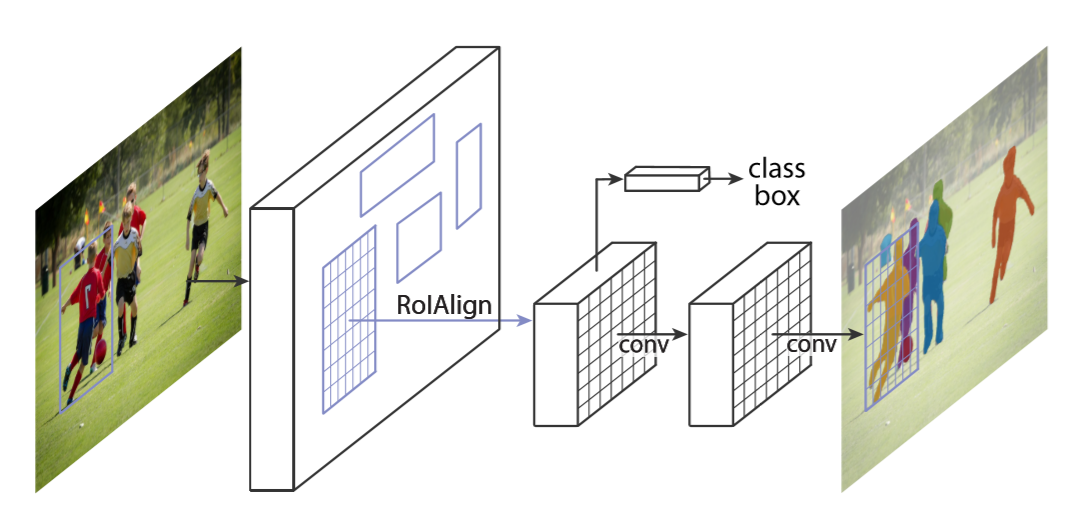
\includegraphics[width=0.5\textwidth]{Img/2-maskRCNN.png}
    \bicaption{实例分割网络Mask R-CNN。}{Instance segmentation network Mask R-CNN.}
    \label{fig:maskRCNN}
\end{figure}
Mask R-CNN以广泛应用的目标检测网络Faster R-CNN为原型,并在其基础上增加了进行语义分割任务的分支。Faster R-CNN 是一个
双阶段的目标检测方法,它包括区域候选网络(Region Proposal Networks, RPN)和位置框回归(Bounding Box Regression)两个部分。
在区域候选网络阶段,RPN将用于生成不同尺度锚框(anchor),以在特征图上对检测框进行粗略描述。对于每个锚框,分别进行前景、背景
分类和位置框的回归,输入建议层(Proposal Layer)。在建议层中,按每个锚框前景类别的Softmax得分排序,经过极大值抑制选取得分最高
的固定数目锚框,生成检测框,完成目标定位过程。不同尺度的检测框会输入兴趣区域池化层(ROI Pooling layer),得到固定大小的特征图。
随后特征图分别送入分类与回归两个分支,在分类分支中经全连接层和Softmax层得到该检测框对应各类别的概率,在回归分支中则再次进行
位置框回归,得到更加准确的位置框预测结果。
\begin{figure}[!htbp]
    \centering
    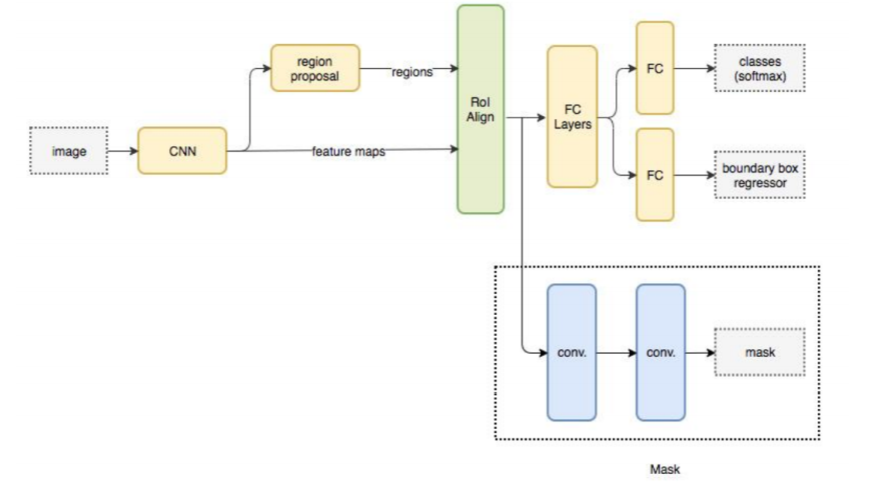
\includegraphics[width=\textwidth]{Img/2-maskRCNNStructure.png}
    \bicaption{Mask R-CNN网络结构。}{Architecture of Mask R-CNN.}
    \label{fig:maskRCNNStructure}
\end{figure}
以Faster R-CNN为基础,Mask R-CNN分为骨干网络和头部网络部分,其结构如图\ref{fig:maskRCNNStructure}所示。骨干网络部分使用ResNet-FPN\citep{he2016deep},负责特征提取。
其中特征金字塔网络(Feature Pyramid Network,FPN)是一种多尺度检测方法,它将ResNet中每个残差块不同尺度的特征图自下而上以
elewise的方式进行整合,不同尺度的特征图经上采样相加,会同时保留低层细节特征和高层全局特征,有利于不同尺度目标的检测。
同时Mask R-CNN提出了兴趣区域对齐算法(RoI Align),将不同层级的特征图输入区域候选网络,消除了兴趣区域池化层带来的的精度损失,
得到了更精准的检测结果,并能够提升分割分支的精度。头部网络部分则是在Fast R-CNN的基础上增加了分割分支,变成前景类别分类、
位置框回归和mask分割三个分支并行的结构,能够完成同步目标检测和实例分割。
\begin{figure}[!htbp]
    \centering
    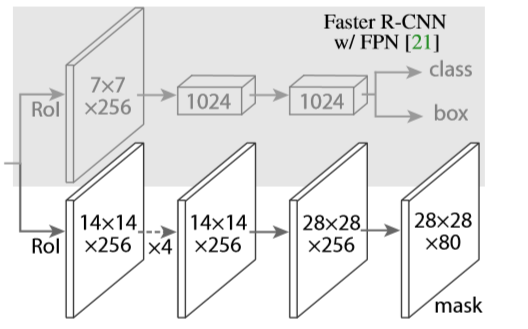
\includegraphics[width=0.35\textwidth]{Img/2-headNetwork.png}
    \bicaption{Mask R-CNN的头部网络结构。}{Network head of Mask R-CNN.}
    \label{fig:headNetwork}
\end{figure}
本文所使用的Mask R-CNN模型使用公开数据集Microsoft COCO\citep{lin2014microsoft}训练,能够检测多达80个类别的物体。
对于第$k$帧中的输入彩色图像$C_{k}$,我们可以获得两个输出:
{
\setlist[enumerate]{}% restore default behavior
\begin{enumerate}[nosep]
    \item 语义mask$m_{k}$。以张与输入图像分辨率相同的单通道图像,其中每个像素的灰度值代表该像素的类别标签。
    \item $J$个对象的检测结果集$\mathbb{R}={r_{0},...,r_{j},...r_{J}} $,其中第$j$个目标的检测结果可表示为$r_{j}={c_{j},b_{j},s_{j}}$,
    $b_{j}=\left[bu_{j},bv_{j},bw_{j},bh_{j}\right]$,每项分别代表该检测框的左上角坐标和宽度、高度。
    每一项分别代表其类别,边界框和置信度。在语义分割阶段,$s_{j}$过低的目标将被抛弃不用,以此保证每一个参与后续流程的目标检测结果
    都足够可靠,而$c_{j}$和$b_{j}$将用于后续的位姿优化及语义建图。
\end{enumerate}
}

\section{系统框架设计}
\begin{figure}[!htbp]
    \centering
    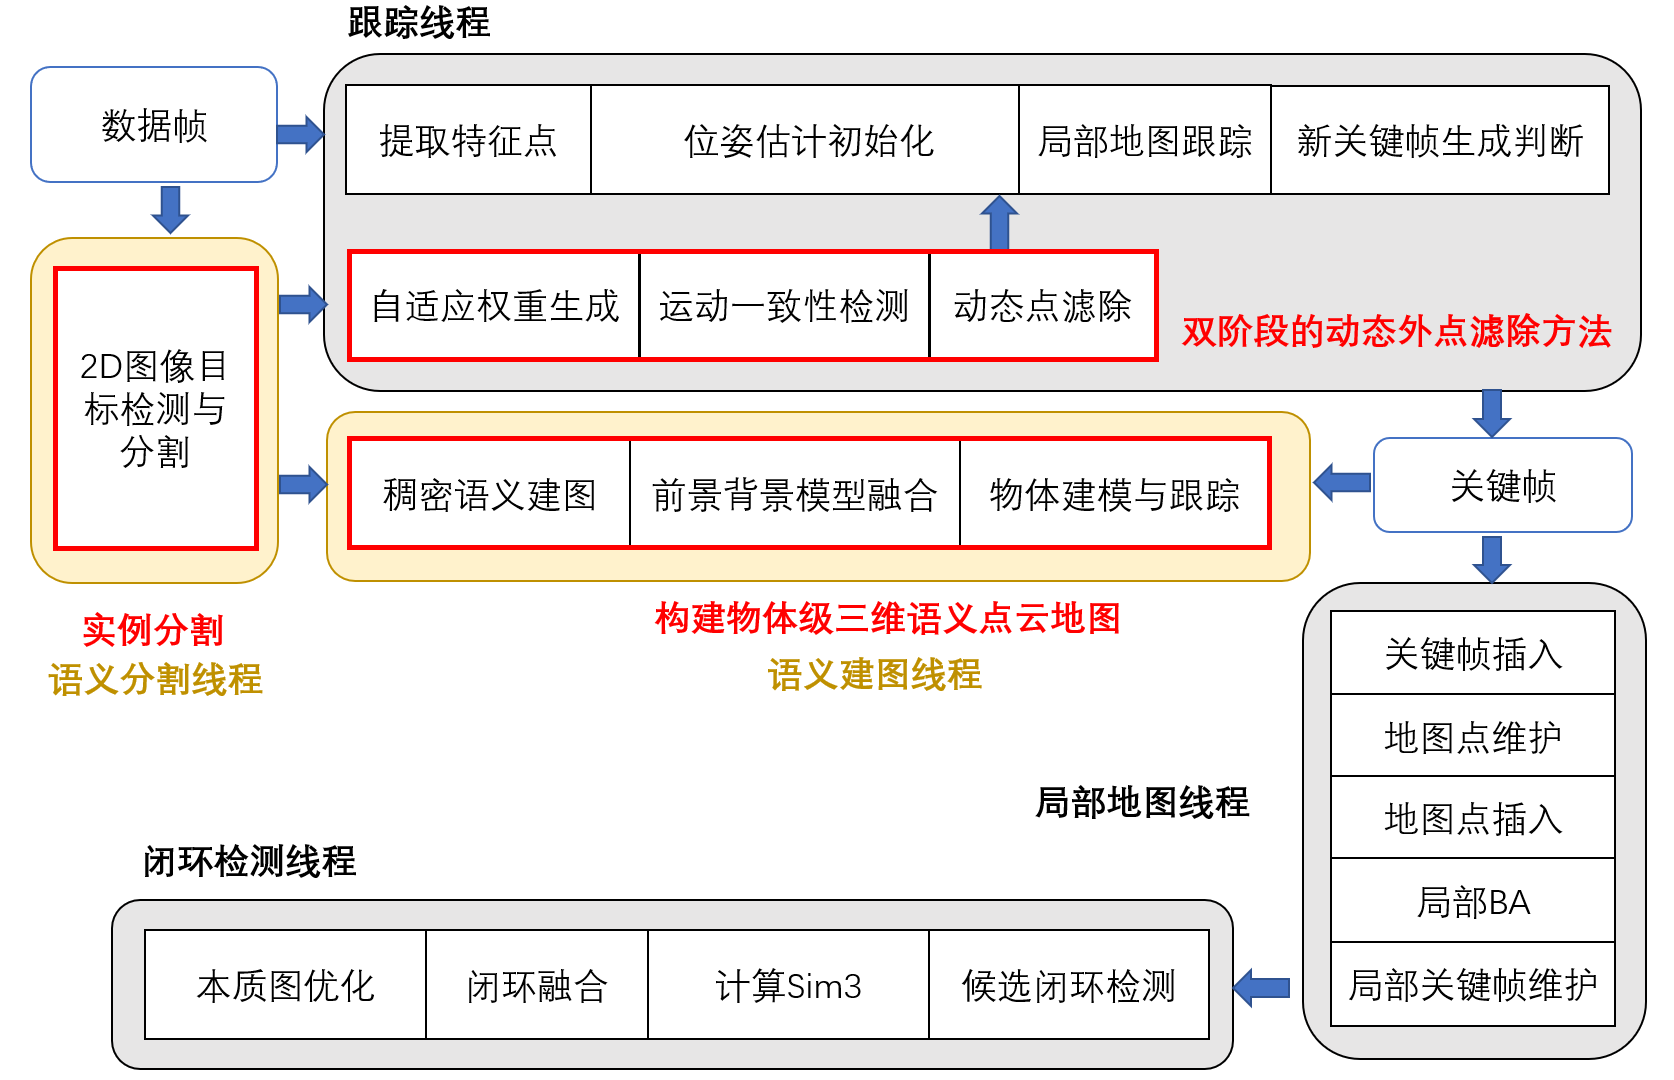
\includegraphics[width=\textwidth]{Img/2-orbPlus.png}
    \bicaption{本文所提出的基于ORB-SLAM2的系统结构。}{ORB-SLAM2-based system architecture proposed in this paper.}
    \label{fig:orbPlus}
\end{figure}
本文将所提出的系统通过深度学习框架Keras将Mask R-CNN结合在了基于特征的视觉SLAM系统ORB-SLAM2中,使得SLAM运行过程中,能够同步
对输入的图像数据进行实例分割,输出目标的类别、置信度、位置框和语义mask。相比于ORB-SLAM2,本文所提出的系统接受RGB-D输入,改进了跟踪线程
并新增了语义建图线程,系统整体共有五个平行的线程:跟踪、局部地图、语义分割、回环闭合和语义建图,具体结构如图\ref{fig:orbPlus}所示。
\begin{figure}[!htbp]
    \centering
    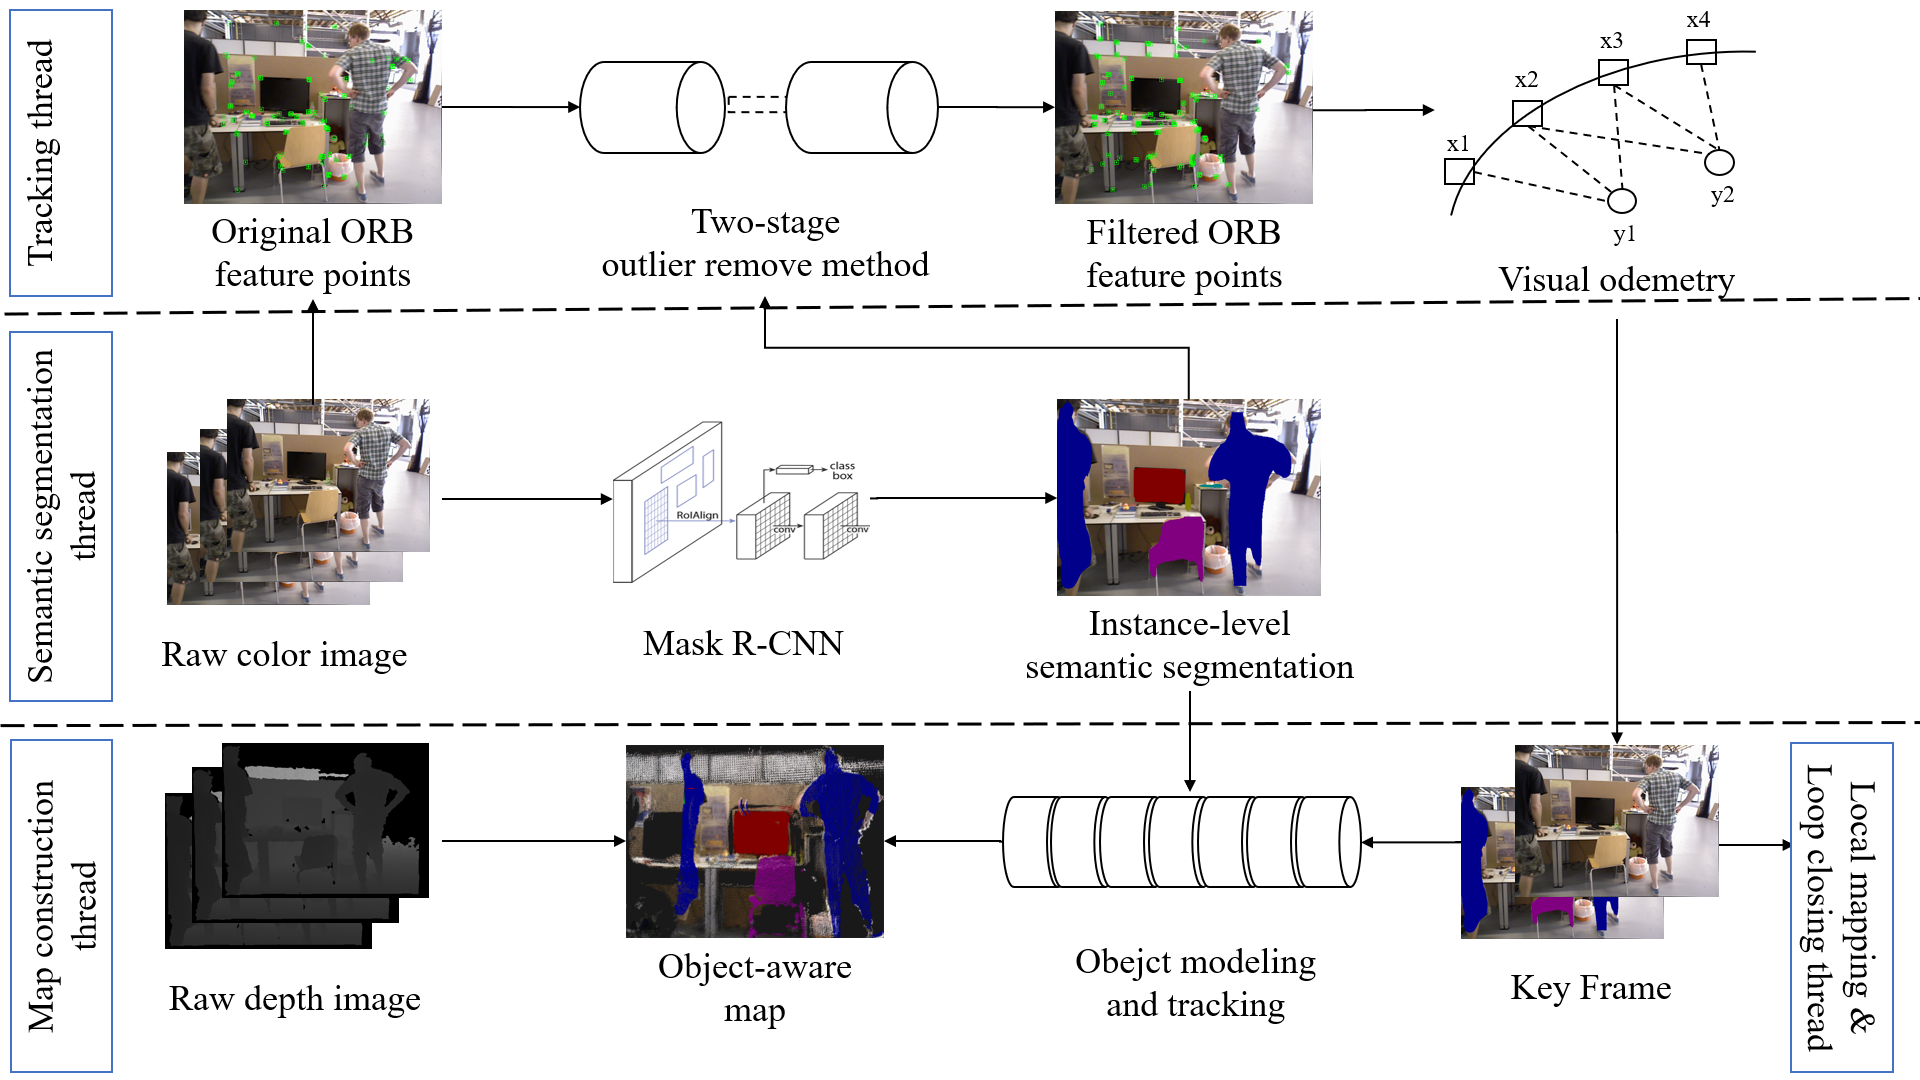
\includegraphics[width=\textwidth]{Img/2-overview.jpg}
    \bicaption{系统工作流程。}{Workflow of our system.}
    \label{fig:overview}
\end{figure}
图如\ref{fig:overview}所示,系统工作流程为:相机捕获RGB-D数据流,每一帧包含彩色图和深度图。输入的彩色图会同步用于语义分割和跟踪线程。
在跟踪线程中,系统对输入的彩色图像提取ORB特征,然后结合语义分割线程输出的预测结果,通过双阶段的动态外点滤除算法
检测动态目标并移除位于动态目标轮廓的特征点,然后对经过滤除的剩余特征点进行特征匹配,用于计算得到相机位姿和路标点估计,
同时会通过一定的策略生成关键帧,分别输入局部地图线程和语义建图线程。局部建图线程与回环闭合线程共同对状态变量进行优化,
得到全局最优的状态估计。语义建图线程会结合语义分割线程输出的预测结果,对其检测到的目标进行建模和跟踪,并随环境变化而更新,
同时会进行2D-3D语义关联,为三维地图中的物体模型赋予不同的语义标签,以建立物体级的语义点云地图。

\section{本章小结}
本章从宏观上介绍了本文的基本框架结构,力求清晰、完整地串联起本文所研究的系统的整体结构和各部分间关联。首先在第一节介绍了SLAM的基本任务和技术要点,第二节介绍了本文所研究的系统所采用的基于特征
的视觉SLAM框架——ORB-SLAM2,第三节介绍了本文所研究的系统采用的网络结构——Mask R-CNN,最后一节阐述了本文所研究系统各个模块
间的关联、交互方式,给出了系统框架设计。

\chapter{动态场景下基于语义信息的位姿估计优化方法}\label{chap:3}
\section{引言}
基于特征的视觉SLAM框架在静态场景下已经具有了较好的鲁棒性和准确度表现,然而在动态场景下的表现却不尽如人意。在场景结构出现变化,如出现走路的人,被抓取移动而的水杯等运动物体时,
场景中静态部分和动态部分在两帧上的投影不满足同一变换关系,因此从图像中静态部分和动态部分提取的特征点不能同时用于两帧间变换矩阵
的计算。换言之,场景中的运动物体为估测相机的运动引入了误差,从而使得SLAM系统整体的状态估计精度降低,甚至会导致跟踪丢失。

针对这一问题,一种直观的解决方案是识别出场景中处于运动状态的物体,将其在二维图像上投影区域内的特征点当做外点移除,从而仅使用
场景中静态部分的特征点进行位姿估计,以提高系统在动态场景下的精确度和鲁棒性。沿袭这一思路,本文提出了一种双阶段的动态外点滤除算法,
此算法结合基于语义类别的自适应权重生成方法和基于极线约束的动态一致性检测方法,能够对于不同类别的物体自适应生成不同的判定条件,
判断其是否处于运动状态,并移除处于运动状态的物体的轮廓内的特征点。本章将就这一方法进行详细介绍,并分析并对比其在公开数据集上的实验结果。

\section{基于极线约束的动态一致性检测方法研究}
\subsection{极线约束}

\begin{figure}[!htbp]
    \centering
    \begin{subfigure}[b]{0.35\textwidth}
      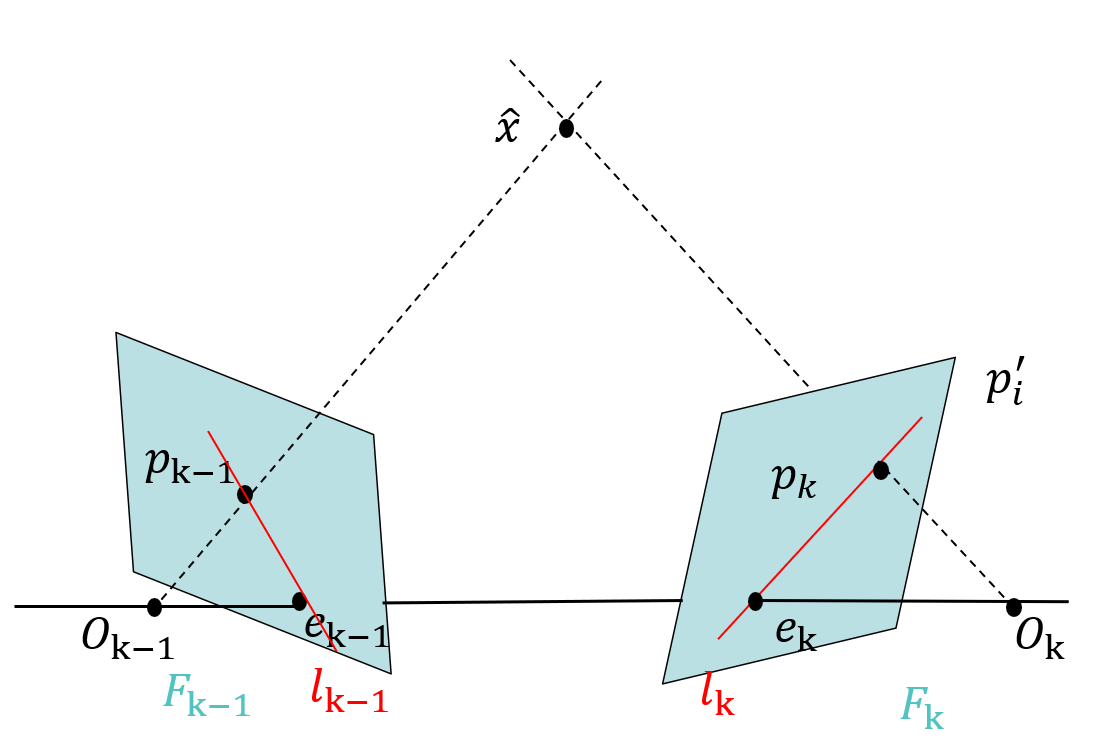
\includegraphics[width=\textwidth]{Img/3-epiplorConstrain.png}
      \caption{}
      \label{fig:epiplorConstrain}
    \end{subfigure}%
    ~% add desired spacing
    \begin{subfigure}[b]{0.35\textwidth}
      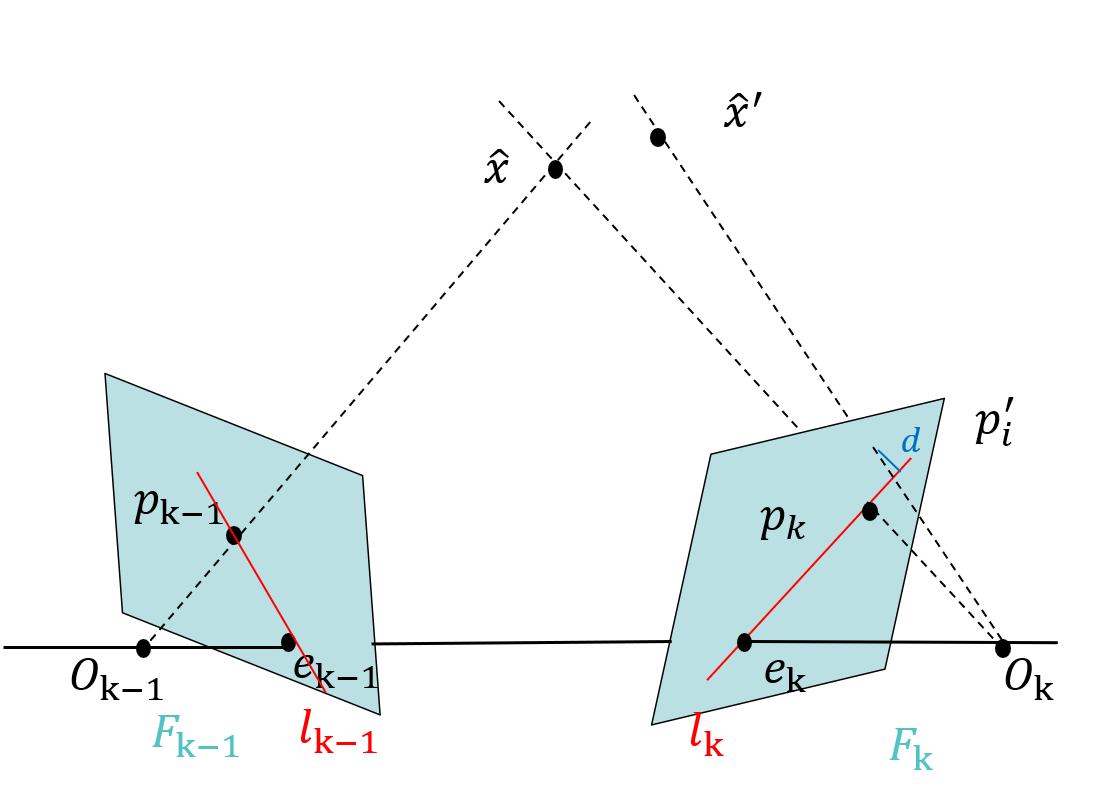
\includegraphics[width=\textwidth]{Img/3-epiplorConstrain2.jpg}
      \caption{}
      \label{fig:epiplorConstrain2}
    \end{subfigure}
    \bicaption{极线约束示意图。(a) 三维点静止时满足极线约束,(b) 三维点运动时不满足极线约束。}{Illustration of epipolar constraint. (a) The epipolar constraint is satisfied when the 3D point is stationary, and (b) the epipolar constraint is not satisfied when the 3D point is in motion.}
    \label{fig:epiplor}
\end{figure}
极线约束如图\ref{fig:epiplor}所示。根据多视图几何原理\citep{hartley2003multiple},对于相机在移动过程中捕捉的连续两帧图像$F_{k-1}$和$F_{k}$,可以提取和匹配
其中一对特征点$P_{k-1}$,$P_{k}$,在静态场景下,$P_{k-1}$和$P_{k}$对应世界坐标系下同一点$\hat{X}=\left[x,y,z\right]^{T}$。
设两帧相机的光心分别为$O_{k-1}$和$O_{k}$,两帧间的运动表示为转移矩阵$T_{k-1,k}=\left[R|t\right]$。两帧相机光心与特征点的连线
$\vec{O_{k-1}P_{k-1}}$、$\vec{O_{k}P_{k}}$会在三维空间中交汇于$\hat{X}=$。

$O_{k-1}$、$O_{k}$、$\hat{X}$三点可以确定一个平面,称作极平面(Epipolar plane),$O_{k-1}$与$O_{k}$两点确定一条直线$O_{k-1}O_{k}$,
称作基线(Baseline),$O_{k-1}O_{k}$与$F_{k-1}$、$F_{k}$分别交于两点$e_{k-1}$、$e_{k}$,称作极点。$e_{k-1}$、$e_{k}$
分别与$P_{k-1}$、$P_{k}$的连线称作极线(Epipolar line),表示为$l_{k-1}$、$l_{k}$,极线也是极平面与$F_{k-1}$和$F_{k}$
的交线。

对于$F_{k-1}$来说,$X$可能位于$\vec{O_{k-1}P_{k-1}}$上任何一点,其在$F_{k-1}$上的投影都是$P_{k-1}$。这些可能的三维点投影在
$F_{k}$上,形成了$\vec{e_{k}P_{k}}$,也就是$F_{k}$的极线$l_{k}$。根据特征点的匹配关系,我们可得而三维点$\hat{X}$在
$F_{k}$上具体的投影位置$P_{k}$,在$\hat{X}$静止不动的前提下,不考虑误差的影响,点$P_{k}$应在极线$l_{k}$上,即极线约束:
$$P_{k}^{T}·l_{k}=0$$
在已知基础矩阵$F$的情况下,根据基础矩阵的定义\citep{hartley2003multiple},有
$$F=e_{k-1}\times H$$
其中$\times$表示叉乘运算,$H$表示$F_{k-1}$与$F_{k}$之间的单应矩阵(Homography),描述了两个平面之间的映射关系。因$e_{k}$
与$P_{k}$同在$l_{k}$上,$l_{k}$又可表示为:
$$l_{k}=e_{k}\times P_{k}$$
因两平面上可以通过单应矩阵变换,可得:
$$P_{k}=HP_{k-1}$$
进而得到:
$$l_{k}=e_{k}\times HP_{k-1}=FP_{k-1}$$
因此极线约束也可写成:
$$P_{k}^{T}·FP_{k-1}=0$$

在静态场景下,同一三维点在两帧上的投影应满足极线约束,$P_{k}$到$l_{k}$的距离$d_{k}$应接近于0。而当三维点处于动态时,如由$\hat{X}$运动至${\hat{X}}^{'}$,极线约束不再满足,
因此,$d_{k}$可以一定程度上反应三维点的运动程度,当$d_{k}$足够大,即有理由认为对应三维点$\hat{X}$处于运动状态。

\subsection{L-K光流法}
由于场景中可能存在处于运动状态物体,通过特征点的匹配集合来计算得出的基础矩阵可能存在误差,因此本算法使用光流法寻找两帧间
像素匹配集合。光流法是基于像素明暗关系对像素的运动进行预测的方法,它能够描述在连续帧间,像素在图像中的运动,通过光流法可预测同一三维点在连续两帧中的位置,获得匹配点坐标。
在本文中,我们选用了经典的L-K光流法(Lucas-Kanade Optical flow)\citep{bouguet2001pyramidal}。

L-K光流法是一种两帧差分的光流估计方法,它假设相机捕获的图像是随时间变化的,对应灰度图$I$是关于时间$t$的函数,可表示为$I_{t}$。
对于三维点$\hat{X}$,在t时刻在图像上的投影可表示为齐次坐标
$$\widetilde{P_{t}}=\left[u,v,1\right]$$
它的灰度值可表示为
$$I(u,v,t)$$
设连续两帧之间该点坐标和时间变化量分别为$du$、$dv$、$dt$,则在经时长为$dt$的变化后,该点可表示为:
$$\widetilde{P_{t+dt}}=\left[u+du,v+dv,1\right]$$
对应的,其灰度值可表示为
$$I(u+du,v+dv,t+dt)$$
光流法的计算基于灰度不变假设,即同一个三维点在不同时刻图像上的投影,其灰度值是保持不变的。据此可以得出:
$$I(u,v,t)=I(u+du,v+dv,t+dt)$$
若两帧间运动量足够小,则可通过泰勒展开进行近似:
$$I(u+du,v+dv,t+dt)\approx I(u,v,t)+\frac{\partial I}{\partial u}du+\frac{\partial I}{\partial v}dy+\frac{\partial I}{\partial t}dt$$
由此得出:
$$\frac{\partial I}{\partial u}du+\frac{\partial I}{\partial v}dy+\frac{\partial I}{\partial t}dt=0$$
进一步变形可得:
$$\frac{\partial I}{\partial u}\frac{du}{dt}+\frac{\partial I}{\partial v}\frac{dv}{dt}=-\frac{\partial I}{\partial t}$$
其中,$\frac{\partial I}{\partial u}$和$\frac{\partial I}{\partial v}$分别为$I(u,v,t)$沿$u$、$v$方向的梯度,$\frac{du}{dt}$
和$\frac{dv}{dt}$分别为像素点$P_{t}$沿$u$、$v$方向运动的速度。将$\frac{\partial I}{\partial u}$和$\frac{\partial I}{\partial v}$
记作$\mathcal{G}=\left[G_{u},G_{v}\right]^{T}$、$\frac{\partial I}{\partial t}dt$记作$G_{t}$、$\frac{du}{dt}$
和$\frac{dv}{dt}$记作$\mathcal{V}=\left[V_{u},V_{v}\right]^{T}$,则上式可以写成:
$$
\mathcal{G}^{T}\cdot \mathcal{V}=
\left[G_{u},G_{v}\right]
\left[
\begin{tabular}{@{}c@{}}
    $V_{u}$ \\ $V_{v}$\\
\end{tabular}
\right]
=
G_{u}V_{u}+ G_{v}V_{v}
=
-G_{t}
$$

发生运动后像素点的坐标值可以通过该像素的运动速度$V_{u}$和$V_{v}$得出,但上式为二元一次方程,无法求出$V_{u}$和$V_{v}$的数值解,
需要引入额外的约束。在L-K光流法中,引入了空间一致性假设,即认为以$P_{t}$为中心,大小为$w\times w$的邻域内,共有$w^{2}$个像素,
所有像素都具有相同的运动速度$\mathcal{V}=\left[V_{u},V_{v}\right]^{T}$,则对于窗口内的所有像素都有:
$$
\begin{array}{l}
    G_{u_{1}}V_{u}+ G_{v_{1}}V_{v}=-G_{t_{1}} \\  
    G_{u_{2}}V_{u}+ G_{v_{2}}V_{v}=-G_{t_{2}} \\ 
    \vdots\\ 
    G_{u_{w^{2}}}V_{u}+ G_{v_{w^{2}}}V_{v}=-G_{t_{w^{2}}} \\  
\end{array}
$$
可以构造超定方程组:
$$
\left[
\begin{array}{l}
    \mathcal{G}_{1}^{T} \\  
    \mathcal{G}_{2}^{T} \\   
    \vdots\\ 
    \mathcal{G}_{w^{2}}^{T} \\   
\end{array}
\right]
\cdot 
\mathcal{V}
=
-
\left[
\begin{array}{l}
    G_{t_{1}}^{T} \\  
    G_{t_{1}}^{T} \\   
    \vdots\\ 
    G_{t_{w^{2}}}^{T} \\   
\end{array}
\right]
$$
记:
$$
\textbf{G}=
\left[
\begin{array}{l}
    \left[G_{u},G_{v}\right]_{1}\\  
    \left[G_{u},G_{v}\right]_{2} \\   
    \vdots\\ 
    \left[G_{u},G_{v}\right]_{w^{2}} \\   
\end{array}
\right]
,
\textbf{b}=
\left[
\begin{array}{l}
    G_{t_{1}}\\  
    G_{t_{2}} \\   
    \vdots\\ 
    G_{t_{w^{2}}} \\   
\end{array}
\right]
$$
可将上述方程组写作:
$$\textbf{G}\cdot\textbf{V}=-\textbf{b}$$
上式可以通过最小二乘法求解,得到像素点$P_{t}$运动速度:
$$
\mathcal{V}=-(\textbf{G}^{T}\textbf{G})^{-1}\textbf{G}^{T}\textbf{b}
$$
根据像素点的运动速度,容易计算出在相机运动后,该像素出现的坐标。在连续两帧$F_{k-1}$、$F_{k}$中,对$F_{k-1}$中的角点使用L-K光流法
跟踪其运动,则可以得到在$F_{k}$上的对应角点集合。因此,可以得到两帧的匹配点集合$\mathbb{P}_{k-1}$、$\mathbb{P}_{k}$。
\subsection{动态一致性检测}
根据上述L-K光流法,可以得出两帧直之间的匹配点集$\mathbb{\widetilde{P}}_{k-1}$、$\mathbb{\widetilde{P}}_{k}$,通过八点法算法,利用匹配点集计算基础矩阵$F$,
具体方法为,对于一对以齐次坐标表示的匹配点$\widetilde{P_{k-1}}=\left[u_{k-1},v_{k-1},1\right]^{T}$和$\widetilde{P_{k}}=\left[u_{k},v_{k},1\right]^{T}$,根据对极几何关系可得:
$$\widetilde{P_{k-1}}^{T}F\widetilde{P_{k}}=0$$
将$F$写成矩阵形式可得:
$$
\left[
\begin{array}{ccc}
    u_{k-1} & v_{k-1} & 1\\
\end{array}
\right]
\left[
\begin{array}{ccc}
    f_{11} & f_{12} & f_{13}\\
    f_{21} & f_{22} & f_{23}\\
    f_{31} & f_{32} & f_{33}\\
\end{array}
\right]
\left[
\begin{array}{l}
    u_{k}\\
    v_{k}\\
    1\\
\end{array}
\right]
=0
$$
将其展开可得到:
$$u_{k}u_{k-1}f_{11}+u_{k}v_{k-1}f_{12}+u_{k}f_{13}+v_{k}u_{k-1}f_{21}+v_{k}v_{k-1}f_{22}+v_{k}f_{23}+u_{k-1}f_{31}+v_{k-1}f_{32}+f_{33}=0$$
将$F$写成向量形式:
$$\mathcal{f}=
\left[
\begin{array}{ccccccccc}
    f_{11} & f_{12} & f_{13} & f_{21} & f_{22} & f_{23} & f_{31} & f_{32} & f_{33}\\
\end{array}
\right]
$$
上式可写成:
$$
\left[
\begin{array}{ccccccccc}
    u_{k}u_{k-1} & u_{k}v_{k-1} & u_{k} & v_{k}u_{k-1} & v_{k}v_{k-1} & v_{k} & u_{k-1} & v_{k-1} & 1\\
\end{array}
\right]
\mathcal{f}
=0
$$
设匹配点集$\mathbb{\widetilde{P}}_{k-1}$、$\mathbb{\widetilde{P}}_{k}$中含有$n$个匹配点对,用其可构造方程组:
$$
\textbf{A}\mathcal{f}=
\left[
\begin{array}{ccccccccc}
    u_{k}^{1}u_{k-1}^{1} & u_{k}^{1}v_{k-1}^{1} & u_{k}^{1} & v_{k}^{1}u_{k-1}^{1} & v_{k}^{1}v_{k-1}^{1} & v_{k}^{1} & u_{k-1}^{1} & v_{k-1}^{1} & 1\\
    \vdots\\
    u_{k}^{n}u_{k-1}^{n} & u_{k}^{n}v_{k-1}^{n} & u_{k}^{n} & v_{k}^{n}u_{k-1}^{n} & v_{k}^{n}v_{k-1}^{n} & v_{k}^{n} & u_{k-1}^{n} & v_{k-1}^{n} & 1\\
\end{array}
\right]
\mathcal{f}
=0
$$
在存在唯一解的情况下,$\textbf{A}$的秩为8,$\mathcal{f}$可以通过最少八组匹配点对解出。由于噪声影响,$\textbf{A}$的秩可能为9,
此时可以求$\mathcal{f}$的最小二乘解,具体方法分求线性解和奇异性约束两步。
\textbf{\emph{求线性解}}

首先对\textbf{A}进行SVD分解求得基本线性解:
$$\textbf{A}=\textbf{U}\textbf{D}\textbf{V}^{T}$$
$\textbf{V}$的最后一列矢量即为$\textbf{A}$最小奇异值对应的奇异向量,也是使得$\|\textbf{A}\mathcal{f}\|$最小的$\mathcal{f}$的解矢量。
\textbf{\emph{奇异性约束}}

得到基本解矢量后,为其增加奇异性约束,确保$F$的奇异性。求最终解为$F^{*}$,满足:
$$
\begin{aligned}{2}
    \min_{F^{*}} \quad & \left \|F-F^{*} \right \| \\
    \mbox{s.t.}\quad & det(F^{*})=0
\end{aligned}
$$
通过SVD分解可求出$F^{*}$,若$F=\textbf{U}\textbf{D}\textbf{V}^{T}$,$\textbf{D}=diag(r,s,t)$,满足$r\geq s \geq t$,
则$F$的最优解为:
$$F^{*}=Udiag(r,s,0)V^{T}$$

为方便描述,之后将八点法求得的基础矩阵最优解$F^{*}$仍记为$F$。求得$F$后,可以计算出像素点$P_{k-1}$对应的极线$l_{k}=\left[x,y,z\right]^{T}$,
进而计算出其匹配点$P_{k}$到$l_{k}$的距离:
$$
d=\frac{\left| P_{k}^{T}FP_{i-1} \right|}{\sqrt{\left \| x^{2}+y^{2}\right \|}}
$$

若$d$超过一定阈值,则认为点$P_{k}$对应的三维点可能处于运动状态,标记$P_{k}$为潜在运动外点。
\section{基于语义类别的自适应权重生成方法研究}
我们注意到,在实际室内场景下,不同种类的物体处于运动状态的可能性也不相同。比如“人”这一类别经常自发行走、活动,很容易处于运动状态;
“椅子”、“水杯”等物体有一定可能性因人为移动等原因而发生移动;而“显示器”,“桌子”等类别的物体,则几乎全程是静止的。因此,
对于不同类别的物体,在相同条件下判断它是否处于运动状态的标准也应有所不同。

本文提出了一种基于先验知识的运动可能性概念,用于自适应地根据目标类别检测结果生成运动状态判定阈值。对于每一类目标,
我们分别为其设置了先验权重$w$,表示这个类别的物体处于运动状态的可能性,数值越大表示这一类别
的物体更倾向于处于静止状态中,特别地,为0表示被预测为此类别的物体不会发生运动,将不参与动态外点的检测过程。
对于当前帧$F_{k}$,在经语义分割模块获取其实例分割结果后,对于检测到的第$j$个目标$r_{j}$,系统将自适应地生成此目标的运动判断阈值:
$$T_{j}=w_{c_{j}}*T_{0}$$
其中$T_{0}$是预设的基础运动判定阈值。$T_{j}$将用于二次判断运动一致性检测阶段得到的潜在运动外点是否处于运动状态,对于位于此
物体区域内的一个像素点$P_{k}$,若其到对应极限的距离满足
$$d>T_{j}$$
则认为此点处于运动状态。

可见,$w$越大类别的物体,在先验假设中认为其更倾向于保持静止,在运动点判定阶段,也自适应地生成了更严苛的判定条件,更不容易
被判断为运动动态。

\section{双阶段的动态外点滤除算法}
\begin{figure}[!htbp]
    \centering
    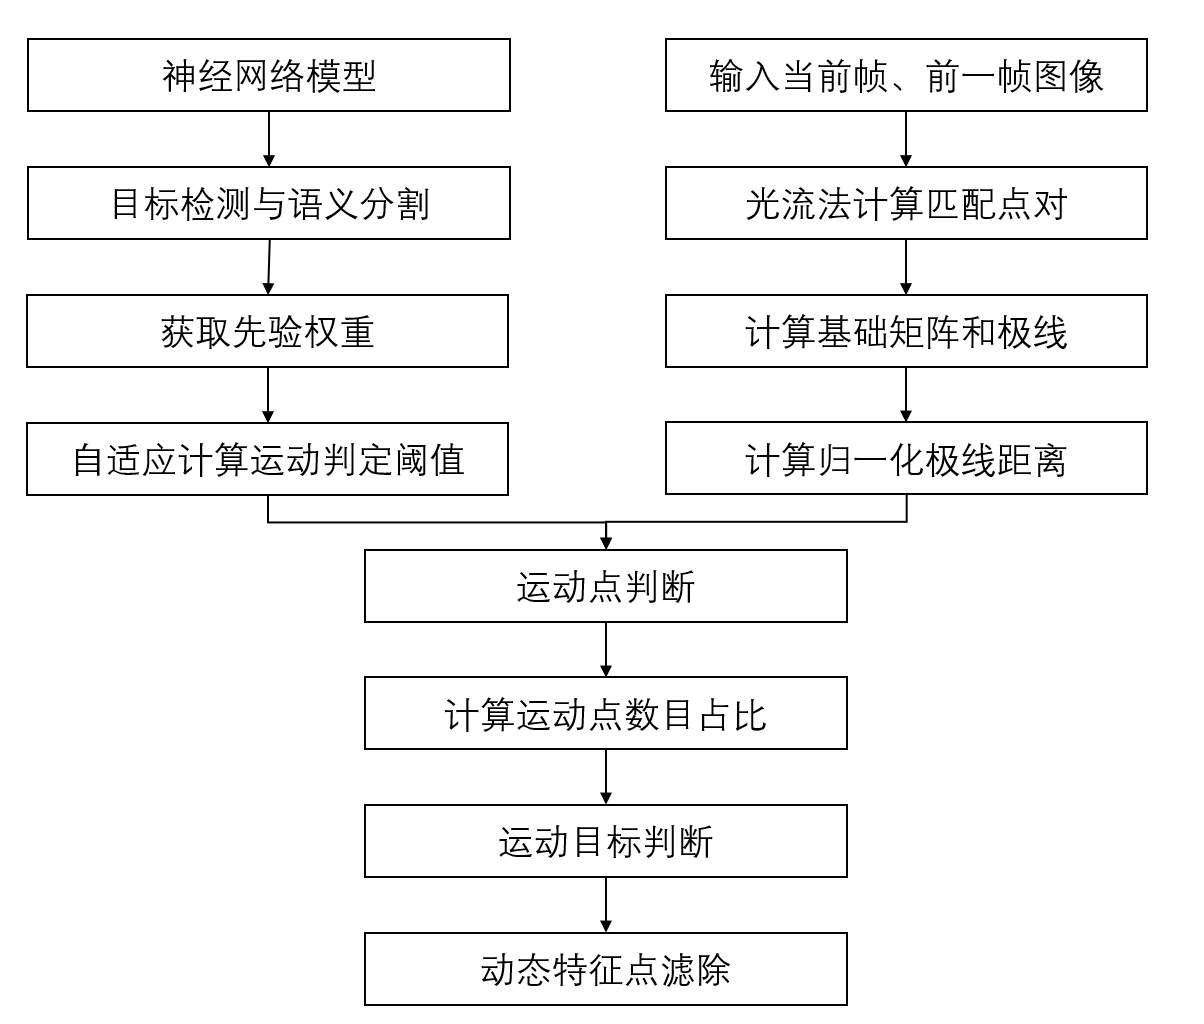
\includegraphics[width=0.6\textwidth]{Img/3-filterflow.png}
    \bicaption{双阶段的动态外点滤除算法流程。}{Workflow of the two-stage dynamic outlier filtering algorithm.}
    \label{fig:filterflow}
\end{figure}
基于以上研究,本文提出了一种双阶段的动态外点滤除算法,结合基于语义类别的自适应权重生成方法和基于极线约束的动态一致性检测方法,
自适应调整不同类别物体的动态点判断阈值,让运动目标检测过程更加平滑,同时结合语义分割结果,能够更精确地仅滤除运动目标范围内的特征点,算法流程如图\ref{fig:filterflow}所示。

在第一阶段,结合语义分割模块预测得到的实例分割结果,系统将通过自适应权重生成方法为其生成运动判断阈值。在第二阶段,将采用运动一致性
检测算法,首先通过L-K光流得到匹配点集并计算得出基础矩阵,并筛选出运动外点。对于每一个检测到的目标$r_{j}$,其位置框$b_{j}$为矩形区域,
对于匹配点集中的点$P_{k}=(u,v)$,若满足:
\begin{equation} 
    \adddotsbeforeeqnnum%
    \begin{cases}
        bu_{j}\geq u\geq bu_{j}+bw_{j}\\
        bv_{j}\geq v\geq bv_{j}+bh_{j}\\
        m(u,v)=c_{j}\\ 
    \end{cases}
\end{equation}
则认为$P_{k}$是此物体的一个前景点,而若$P_{k}$同时满足$d_{k}>T_{j}$,则认为此点是一运动点。统计一个目标所含前景点和运动点的数目,
表示为$N_{object}$和$N_{moving}$,计算运动点占前景点的比例:
$$\eta_{moving}=\frac{N_{moving}}{N_{object}}$$
若$\eta_{moving}$大于一个预设比例阈值$\xi$,我们认为物体$r_{j}$处于运动状态,继而将所有属于其前景部分的特征点移除,以此确保
最大程度上减小环境中动态物体的影响,并减少非目标前景的静态点的误移除。

此算法具体描述为:
\begin{algorithm} %算法开始 
    \small
    \caption{动态外点滤除算法} \label{alg1} %算法的标签 
    \begin{algorithmic}[1] %此处的[1]控制一下算法中的每句前面都有标号 
    \Procedure{滤除后的特征点集合}$\mathbb{f}_{k}$
    %\REQUIRE 当前帧, $F_{k}$;上一帧, $F_{k-1}$;物体检测结果集合$\mathbb{R}$;基础运动判定阈值$T_{0}$
    %\ENSURE 滤除后的特征点集合,$\mathbb{f}_{k}$;
    % if-then-else 
    \State ${\mathbb{f}}_{k}^{'}=ExtractORBKeyPoints(F_{k})$
    \State $p_{k},p_{k-1}=CalOpticalFlowM atching(F_{k-1},F_{k})$
    \State $F=FindFundamentalMat(p_{k-1},p_{k})$
    \For{each $r_{j}$ in $\mathbb{R}$}
    \State $T_{j}=CalMotionT resh(w_{c_{j}},T_{0})$
    \For{each $p_{k}^{i}$ in $r_{j}$}
    \If{$IsForeground(p_{k}^{i},b_{j},m)$}
    \State $l^{i}=CalEpipolarLine(F,p_{k-1}^{i})$
    \State $d^{i}=CalDistoEpipolarLine(l^{i},p_{k}^{i})$
    \If{$d_{k}$ bigger than $T_{k}$}
    \State $N_{moving}\gets N_{moving}+1$
    \EndIf
    \State $N_{object}\gets N_{object}$
    \EndIf
    \EndFor
    \State $\eta_{moving}=CalMovingRatio(N_{moving},N_{object})$
    \If{$\eta_{moving}$大于$\xi$}
    \For{each $f_{i}^{k}$ in $F_{i}^{'}$}
    \If{$IsForeground(f_{i}^{k},b_{j},m)$}
    \State $F_{i}=RemoveOutliers(F_{i}^{'},f_{i}^{k})$
    \EndIf
    \EndFor
    \EndIf
    \EndFor
    \EndProcedure
    \end{algorithmic} 
\end{algorithm}


\section{实验结果与分析}
\subsection{轨迹误差评测}
我们使用TUM RGB-D数据集\citep{sturm2012benchmark}测试了双阶段的动态外点滤除算法在动态环境下对相机位姿估计的优化效果。
TUM RGB-D数据集是由德国慕尼黑工业大学计算机视觉实验室于2012年发布的RGB-D数据集,在当前有着广泛的应用,它使用Microsoft Kinect
以视频帧率(30 Hz)记录,共包含39个序列,每个序列都包含全传感器分辨率(640x 480)下的彩色和深度图像,主要针对纹理丰富的室内办公室场景。

我们选取了了两个场景的片段:
{
\setlist[enumerate]{}% restore default behavior
\begin{enumerate}[nosep]
    \item 走动场景\\高度动态性的以办公区域为主场景,两个人在桌子前后站起、来回走动、坐下。
    \item 对坐场景\\较低动态性以办公区域为主场景,两个人坐在桌子前交谈,辅以手势进行交流,时而小幅度运动。
\end{enumerate}
}

这两个场景都分别使用了四种相机运动方式来记录,包括:
{
\setlist[enumerate]{}% restore default behavior
\begin{enumerate}[nosep]
    \item halfsphere方式\\相机跟随直径为一米的半球的轨迹移动来记录。
    \item xyz方式\\相机沿x、y、z轴移动来记录。
    \item rpy方式\\相机在俯仰角、偏航角、翻滚角上旋转来记录。
    \item static方式\\相机手动保持静态来记录。
\end{enumerate}
}

通过以上四种记录方式记录两个场景,共构成八个序列片段,分别命名为\emph{sitting\_halfsphere}、\emph{sitting\_rpy}、\emph{sitting\_xyz}、\emph{sitting\_static}、\emph{walking\_halfsphere}、\emph{walking\_rpy}、\emph{walking\_xyz}、\emph{walking\_static}其中一些序列是高度动态的,这对于传统的基于特征的视觉SLAM系统来说很难处理。
我们使用这八个片段,测试了本文所提出的位姿估计优化方法,并与此方法的基础SLAM框架ORB-SLAM2实验数据进行了对比,对于每个片段
我们都运行了五次,并对结果取平均值。在我们的实验中,
我们设置“人”这一类别的先验权重为1,“椅子”这一类别的先验权重为5,其余如“键盘”、“显示器”等类别为0。

在实验数据的评估方面,我们使用了绝对轨迹误差(Absolute Trajectory Error,ATE)和相对位姿误差(d Relative Pose Error,RPE)作为评价标准,
其中,绝对轨迹误差能够评估相机轨迹的全局一致性,而相对位姿误差可以评估相机位姿在平移和旋转两方面的误差漂移。我们对整个轨迹
按固定步长采样,计算每个采样点的误差,并以四种方式计算得出全局误差:
{
\setlist[enumerate]{}% restore default behavior
\begin{enumerate}[nosep]
    \item 均方根误差(Root Mean Square Error,RMSE)\citep{pathak2016context}\\表示所有误差项的均方根。
    \item 均值\\表示估计所有误差项的均值。
    \item 中位数\\表示所有误差项的中位数。
    \item 标准差(Standard Deviation,S.D.)\\表示所有误差项的标准差。
\end{enumerate}
}
\begin{table*}[!htbp]
    \bicaption{绝对轨迹误差对比结果。}{RESULTS OF METRICS ABSOLUTE TRAJECTORY ERROR (ATE).}
    \label{tab:ATE}
    \centering
    \footnotesize% fontsize
    \setlength{\tabcolsep}{8pt}% column separation
    \renewcommand{\arraystretch}{1.3}%row space 
    \begin{tabular}{l|cccc|cccc}
        \hline
        & \multicolumn{4}{c|}{ORB SLAM2}                                         & \multicolumn{4}{c}{本文所提出的系统}                                        \\ \hline
        & RMSE            & median          & mean            & std             & RMSE            & median          & mean            & std             \\ \hline
        sitting\_halfsphere & 0.0198          & 0.0127          & 0.0151          & 0.0127          & \textbf{0.0156} & \textbf{0.0122} & \textbf{0.0137} & \textbf{0.0073} \\ \hline 
        sitting\_rpy        & \textbf{0.0197} & \textbf{0.0120} & \textbf{0.0157} & \textbf{0.0120} & 0.0201          & 0.0123          & 0.0158          & 0.0121          \\ \hline
        sitting\_static     & 0.0085          & 0.0071          & 0.0076          & 0.0038          & \textbf{0.0063} & \textbf{0.0048} & \textbf{0.0055} & \textbf{0.0032} \\ \hline
        sitting\_xyz        & \textbf{0.0090} & \textbf{0.0073} & \textbf{0.0079} & \textbf{0.0045} & 0.0101          & 0.0083          & 0.0090          & 0.0046          \\ \hline
        walking\_halfsphere & 0.7057          & 0.5928          & 0.6113          & 0.3527          & \textbf{0.0360} & \textbf{0.0244} & \textbf{0.0300} & \textbf{0.0200} \\ \hline
        walking\_rpy        & 0.8111          & 0.6513          & 0.7091          & 0.3939          & \textbf{0.1448} & \textbf{0.0789} & \textbf{0.1071} & \textbf{0.0773} \\ \hline
        walking\_static     & 0.4237          & 0.3247          & 0.3864          & 0.1739          & \textbf{0.0090} & \textbf{0.0073} & \textbf{0.0081} & \textbf{0.0039} \\ \hline
        walking\_xyz        & 0.7287          & 0.5802          & 0.6463          & 0.3366          & \textbf{0.0197} & \textbf{0.0127} & \textbf{0.0154} & \textbf{0.0112} \\ \hline
        \hline
    \end{tabular}
\end{table*}

\begin{table*}[!htbp]
    \bicaption{相对位姿误差旋转项对比结果。}{RESULTS OF METRIC ROTATIONAL DRIFT (RPE).}
    \label{tab:RPER}
    \centering
    \footnotesize% fontsize
    \setlength{\tabcolsep}{8pt}% column separation
    \renewcommand{\arraystretch}{1.3}%row space 
    \begin{tabular}{l|cccc|cccc}
        \hline
        & \multicolumn{4}{c|}{ORB SLAM2}                                         & \multicolumn{4}{c}{本文所提出的系统}                                        \\ \hline
        & RMSE            & median          & mean            & std             & RMSE            & median          & mean            & std             \\ \hline
        sitting\_halfsphere & \textbf{0.5822} & \textbf{0.4613} & \textbf{0.5119} & \textbf{0.2774} & 0.6497          & 0.5123          & 0.5735          & 0.3052          \\ \hline
        sitting\_rpy        & \textbf{0.7889} & \textbf{0.5852} & \textbf{0.6771} & \textbf{0.4048} & 0.8170          & 0.5939          & 0.6981          & 0.4146          \\ \hline
        sitting\_static     & 0.2878          & 0.2504          & 0.2595          & 0.1244          & \textbf{0.2722} & \textbf{0.2311} & \textbf{0.2437} & \textbf{0.1201} \\ \hline
        sitting\_xyz        & \textbf{0.4701} & \textbf{0.3429} & \textbf{0.3988} & \textbf{0.2490} & 0.4850          & 0.3518          & 0.4115          & 0.2561          \\ \hline
        walking\_halfsphere & 9.5391          & 2.3127          & 6.3003          & 7.1624          & \textbf{0.8587} & \textbf{0.6772} & \textbf{0.7504} & \textbf{0.4160} \\ \hline
        walking\_rpy        & 9.0072          & 2.9693          & 6.1350          & 6.5948          & \textbf{2.4676} & \textbf{0.9672} & \textbf{1.6239} & \textbf{1.8056} \\ \hline
        walking\_static     & 4.2935          & 0.3997          & 1.8289          & 3.8844          & \textbf{0.2745} & \textbf{0.2341} & \textbf{0.2481} & \textbf{0.1167} \\ \hline
        walking\_xyz        & 6.9545          & 2.4975          & 4.7607          & 5.0696          & \textbf{0.6555} & \textbf{0.4329} & \textbf{0.5221} & \textbf{0.3880} \\ \hline
        \hline
    \end{tabular}
\end{table*}
\begin{table*}[!htbp]
    \bicaption{相对位姿误差平移项对比结果。}{RESULTS OF METRIC TRANSLATIONAL DRIFT (RPE).}
    \label{tab:RPET}
    \centering
    \footnotesize% fontsize
    \setlength{\tabcolsep}{8pt}% column separation
    \renewcommand{\arraystretch}{1.3}%row space 
    \begin{tabular}{l|cccc|cccc}
        \hline
        & \multicolumn{4}{c|}{ORB SLAM2}                                         & \multicolumn{4}{c}{本文所提出的系统}                                        \\ \hline
        & RMSE            & median          & mean            & std             & RMSE            & median          & mean            & std             \\ \hline
        sitting\_halfsphere & 0.0227          & 0.0119          & 0.0162          & 0.0159          & \textbf{0.0190} & \textbf{0.0152} & \textbf{0.0168} & \textbf{0.0088} \\ \hline
        sitting\_rpy        & \textbf{0.0248} & \textbf{0.0160} & \textbf{0.0203} & \textbf{0.0143} & 0.0261          & 0.0170          & 0.0214          & 0.0147          \\ \hline
        sitting\_static     & 0.0095          & 0.0075          & 0.0084          & 0.0046          & \textbf{0.0078} & \textbf{0.0060} & \textbf{0.0068} & \textbf{0.0038} \\ \hline
        sitting\_xyz        & \textbf{0.0115} & \textbf{0.0090} & \textbf{0.0100} & \textbf{0.0058} & 0.0125          & 0.0098          & 0.0109          & 0.0060          \\ \hline
        walking\_halfsphere & 0.4451          & 0.0883          & 0.2889          & 0.3386          & \textbf{0.0369} & \textbf{0.0261} & \textbf{0.0306} & \textbf{0.0205} \\ \hline
        walking\_rpy        & 0.4581          & 0.1554          & 0.3105          & 0.3369          & \textbf{0.1230} & \textbf{0.0453} & \textbf{0.0795} & \textbf{0.0921} \\ \hline
        walking\_static     & 0.2388          & 0.0185          & 0.1003          & 0.2167          & \textbf{0.0105} & \textbf{0.0084} & \textbf{0.0094} & \textbf{0.0047} \\ \hline
        walking\_xyz        & 0.3682          & 0.1400          & 0.2514          & 0.2690          & \textbf{0.0245} & \textbf{0.0160} & \textbf{0.0196} & \textbf{0.0136} \\ \hline
        \hline
    \end{tabular}
\end{table*}

测量数据如表\ref{tab:ATE}-表\ref{tab:RPET}所示,可以看出,本文所提出的SLAM系统在走动场景中,相比ORB-SLAM2,无论在绝对轨迹误差还是相对位姿误差
上都取得了量级式的误差降低,这说明了在高度动态的环境下,本文所提出的方法能够显著提升系统的位姿估计精度和鲁棒性。然而,在较低
动态性的对坐场景中,本文所提出的SLAM系统相比于ORB-SLAM2的取得了略微的提升,或二者的数值差异不大,经分析,我们认为导致在轻度动态
场景下提升不够明显这一现象的原因是,动态外点滤除算法减少了用于位姿估计的ORB特征点总数,使得迭代优化过程中没有足够的约束支撑。
另一个不可忽视的原因是,ORB-SLAM2作为当前表现优异的SLAM系统之一,其在静态场景下已经取得了足够高的精度,因此提升空间是十分有限的。

图\ref{fig:trajectory}展示了对于片段\emph{walking\_xyz},ORB-SLAM2和本文所提出的系统的预测以及真值的轨迹可视化对比。

\begin{figure*}[h]
    \centering
    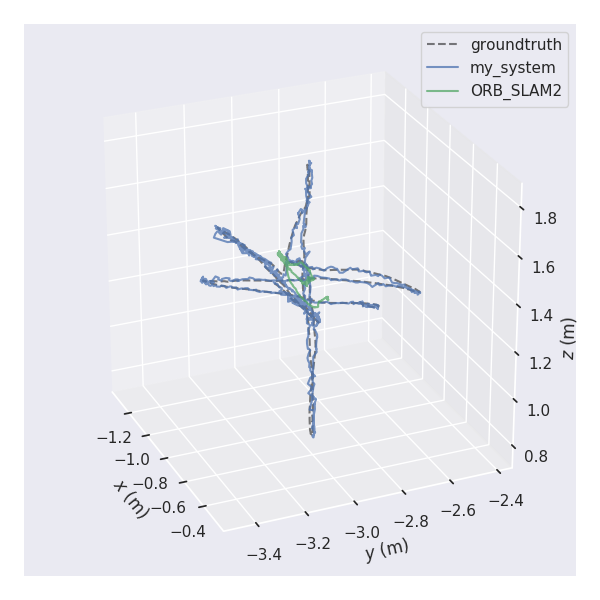
\includegraphics[width=0.31\textwidth]{Img/evo1.png}
    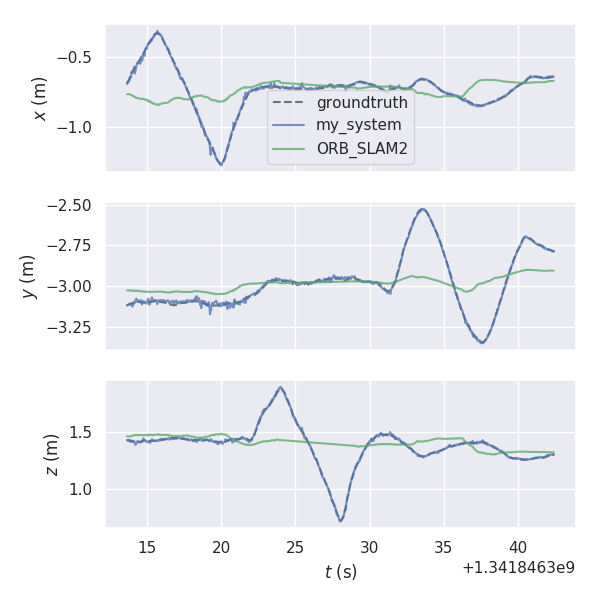
\includegraphics[width=0.31\textwidth]{Img/evo2.png}
    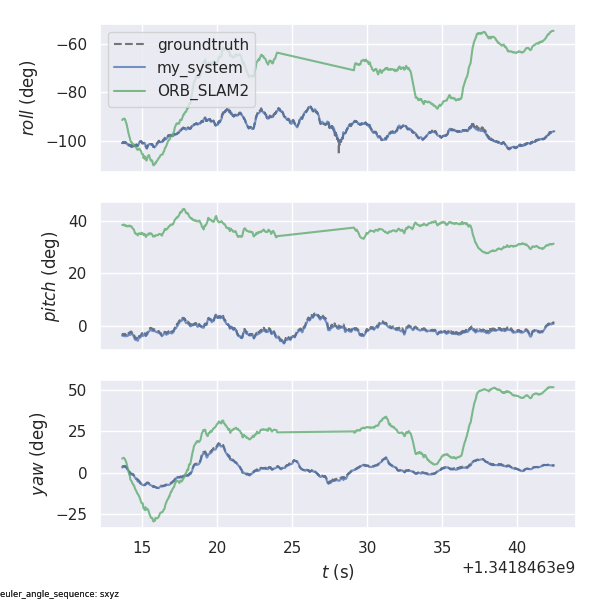
\includegraphics[width=0.31\textwidth]{Img/evo3.png}
    \caption{对于片段\emph{walking\_xyz},ORB-SLAM2和本文所提出的系统的预测以及真值的轨迹可视化对比。}
    \label{fig:trajectory}
  \end{figure*}

本文所提出的SLAM系统也与当前表现最优异的面向动态环境的语义SLAM系统进行了对比,包括DS-SLAM和DynaSLAM。为了避免不同运行环境
引入的实验数据误差,本文直接引用了对比系统原始论文中发布的改进方法和基础方法的测试数据,DS-SLAM、DynaSLAM和本文所提出的方法
都以ORB-SLAM2为基础方法,因此,我们计算了各自改进相对于ORB-SLAM2的提升幅度以进行比较。具体计算方法如下:
$$\rho=\frac{e_{0}-e}{e_{0}}*100$$
其中,$e_{0}$为ORB-SLAM2的误差值,$e$为改进方法的误差值,$\rho$表示误差减少的百分比。
\begin{table*}[!htbp]
    \bicaption{与DS-SLAM的对比结果\citep{YuDS}。}{Comparison of DS-SLAM\citep{YuDS}.}
    \label{tab:DSSLAM}
    \centering
    \footnotesize% fontsize
    \setlength{\tabcolsep}{8pt}% column separation
    \renewcommand{\arraystretch}{1.3}%row space 
    \begin{tabular}{l|ccc|ccc}
        \hline
        & \multicolumn{3}{c|}{DS-SLAM}                                       & \multicolumn{3}{c}{本文所提出的系统}                                    \\ \hline
        & RPET & RPER & ATE            & RPET         & RPER         & ATE            \\ \hline
sitting\_static     & 17.61                    & 5.07                  & \textbf{25.94} & \textbf{18.39}           & \textbf{5.41}         & 25.45          \\ \hline
walking\_halfshpere & 91.62                    & 88.96                 & 93.76          & \textbf{91.70}           & \textbf{91.00}        & \textbf{94.89} \\ \hline
walking\_rpy        & 64.64                    & 62.82                 & 48.97          & \textbf{73.14}           & \textbf{72.60}        & \textbf{82.15} \\ \hline
walking\_static     & 95.27                    & 93.09                 & 97.91          & \textbf{95.59}           & \textbf{93.61}        & \textbf{97.88} \\ \hline
walking\_xyz        & 91.93                    & 89.32                 & 96.71          & \textbf{93.35}           & \textbf{90.57}        & \textbf{97.30} \\ \hline
        \hline
    \end{tabular}
\end{table*}

\begin{table*}[!htbp]
    \bicaption{与DynaSLAM的对比结果\citep{BertaDynaSLAM}。}{Comparison of DynaSLAM\citep{BertaDynaSLAM}.}
    \label{tab:DynaSLAM}
    \centering
    \footnotesize% fontsize
    \setlength{\tabcolsep}{8pt}% column separation
    \renewcommand{\arraystretch}{1.3}%row space 
    \begin{tabular}{l|c|c}
        \hline
        & \multicolumn{1}{c|}{DynaSLAM}         & \multicolumn{1}{c}{本文所提出的系统}           \\ \hline
      %  & DynaSLAM          & our system        \\ \hline
        sitting\_halfsphere & 15                & \textbf{21.0869}  \\ \hline
        sitting\_xyz        & -66.6667          & \textbf{-12.7556} \\ \hline
        walking\_halfsphere & 92.87749          & \textbf{94.8932}  \\ \hline
        walking\_rpy        & \textbf{94.71299} & 82.1502           \\ \hline
        walking\_static     & 93.33333          & \textbf{97.8809}  \\ \hline
        walking\_xyz        & 96.73203          & \textbf{97.2958}  \\ \hline
        \hline
    \end{tabular}
\end{table*}
表\ref{tab:DSSLAM}展示了与DS-SLAM在绝对轨迹误差、相对位姿误差上比较结果,误差项使用RMSE计算,其中RPET和RPER分别代表相对位姿误差
的平移和旋转误差偏移。表\ref{tab:DynaSLAM}展示了与DynaSLAM在绝对轨迹误差项上的提升对比,误差项使用RMSE计算。
这些数据证明了本文所提出的优化方法在几乎所有项上都取得了比当前最优秀的SLAM方法更多的提升,这从侧面证明了本文所提出的有效性。

\subsection{特征点滤除效果评测}
\begin{figure}[!htbp]
    \centering
    \begin{subfigure}[b]{0.35\textwidth}
      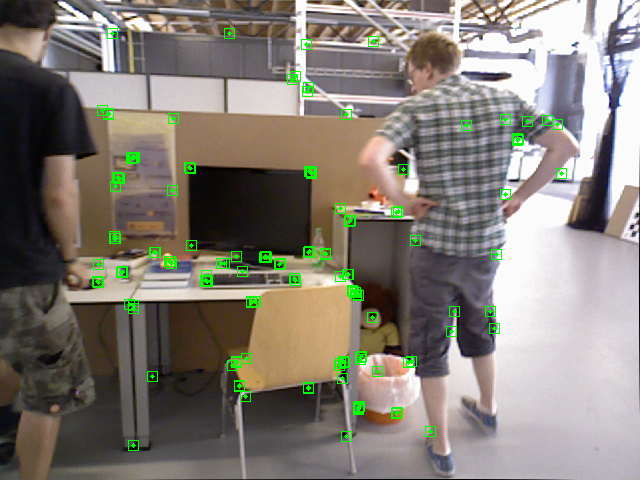
\includegraphics[width=\textwidth]{Img/orb_63.png}
      \caption{}
      \label{fig:orb_63}
    \end{subfigure}%
    ~% add desired spacing
    \begin{subfigure}[b]{0.35\textwidth}
      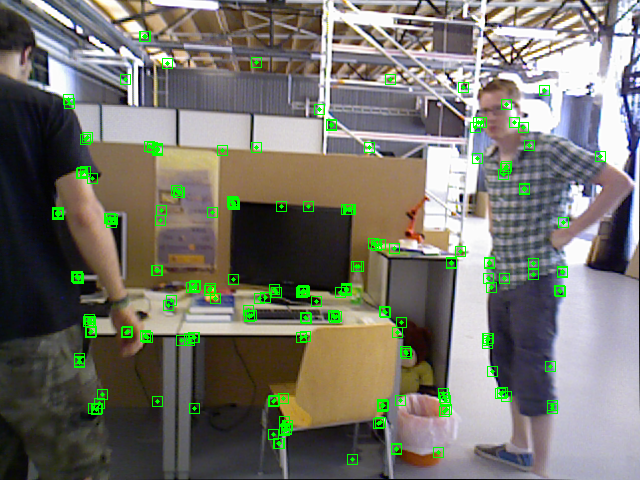
\includegraphics[width=\textwidth]{Img/orb_87.png}
      \caption{}
      \label{fig:orb_87}
    \end{subfigure}
    \\% line break
    \begin{subfigure}[b]{0.35\textwidth}
      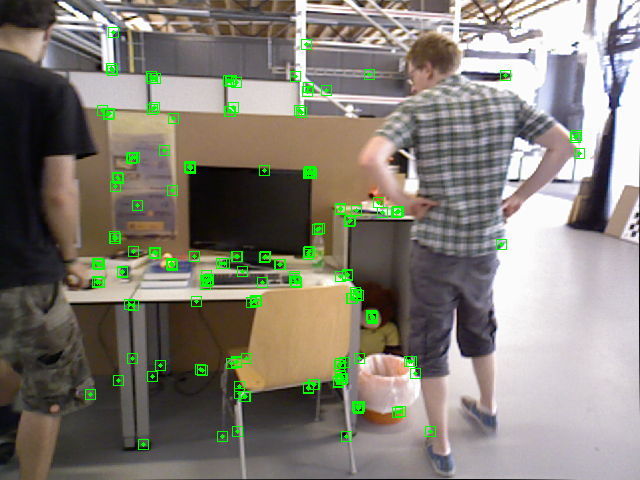
\includegraphics[width=\textwidth]{Img/filter_63.png}
      \caption{}
      \label{fig:filter_63}
    \end{subfigure}%
    ~% add desired spacing
    \begin{subfigure}[b]{0.35\textwidth}
      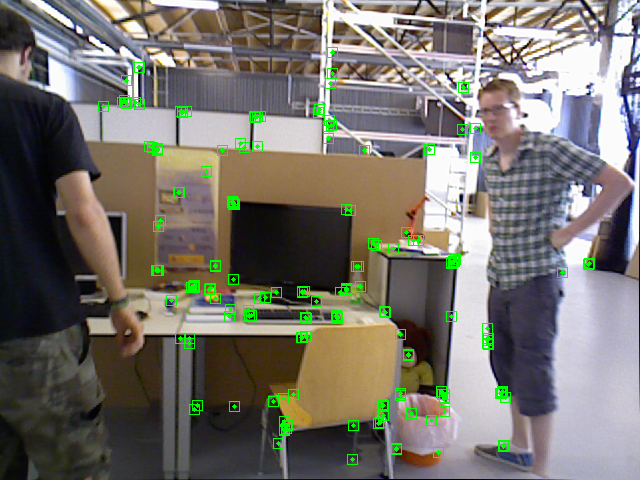
\includegraphics[width=\textwidth]{Img/filter_87.png}
      \caption{}
      \label{fig:filter_87}
    \end{subfigure}
    \bicaption{片段\emph{walking\_xyz}上特征点滤除效果对比。(a) 第63帧原ORB特征点提取结果,(b) 第87帧原ORB特征点提取结果,(c) 第63帧滤除后的ORB特征点,(d) 第87帧滤除后的ORB特征点。}{Comparison of feature point filtering effect on the segment \emph{walking\_xyz}. (a) Original ORB feature point extraction result at frame 63, (b) Original ORB feature point extraction result at frame 87, (c) ORB feature point filtered at frame 63, (d) ORB feature point filtered at frame 87}
    \label{fig:featurefilter}
\end{figure}

图\ref{fig:featurefilter}展示了经动态外点滤除算法作用前后的ORB特征点可视化对比效果,本实验选取了片段\emph{walking\_xyz}上的第63帧
和第87帧,可以看出,对于图中处于运动状态的两个人物,其轮廓内的特征点都被滤除,仅有从静态背景中提取的特征点参与了后续位姿估计的计算。

\section{本章小结}
本章主要介绍了对于动态场景下基于语义信息的位姿估计优化方法的研究,详细描述了本文提出的两阶段动态外点滤除算法,介绍了
基于语义类别的自适应权重生成方法和基于极线约束的动态一致性检测方法两个阶段涉及的基础原理,以及算法具体的流程。最后,展示并分析了
在公开数据集上的实验结果,与当前优秀的SLAM系统ORB-SLAM2、DS-SLAM、DynaSLAM进行了对比,证明了本文所提出方法的有效性。
\chapter{语义地图的构建和表示方法}\label{chap:4}
\section{引言}
传统基于特征的视觉SLAM框架仅能构建包含三维空间信息的几何地图,对于环境的表达能力有所限制。在增强现实应用中,感知环境的语义信息,
获取某一空间位置存在什么种类的物体,能够帮助增强现实系统更精准地将虚拟信息融合进实际环境,优化物理遮挡效果,提供更好的真实感体验,因此探究
语义地图的构建和表示方法对增强现实应用来说具有很高的研究价值。

本章讨论了两种语义地图的构建和表示方法:基于局部特征的预置语义库地图和基于语义SLAM的物体级三维语义点云地图,分别侧重于
室外场景和动态场景对各自的建图能力进行了算法研究,给出并分析了语义建图的实验结果。
\section{特征级语义地图的构建和表示}\label{cha_41}
增强现实系统的运行依赖于对环境的感知,实现方式主要包括基于GPS的感知方法、基于二维标识的感知方法和基于环境理解的感知方法。在
室外环境下,GPS往往存在3~5m的定位误差,依靠GPS进行虚实融合会存在不可避免的偏移现象。基于二维标识的感知方法往往需要进行预先
布置,依靠二维码等方式进行识别不包含对环境的理解。基于环境理解的感知方法往往不适用于室外大尺度场景下,易受干扰,不够鲁棒。因此,
本节研究了一种基于局部特征的预置语义库地图的方法,预先建立在室外场景的语义库地图,通过特征识别和GPS相结合的方式进行识别定位,从而
提升增强现实系统对于室外环境的理解能力,图\ref{ismar}展示了基于此地图的增强现实系统工作流程。
\begin{figure}[!htbp]
    \centering
    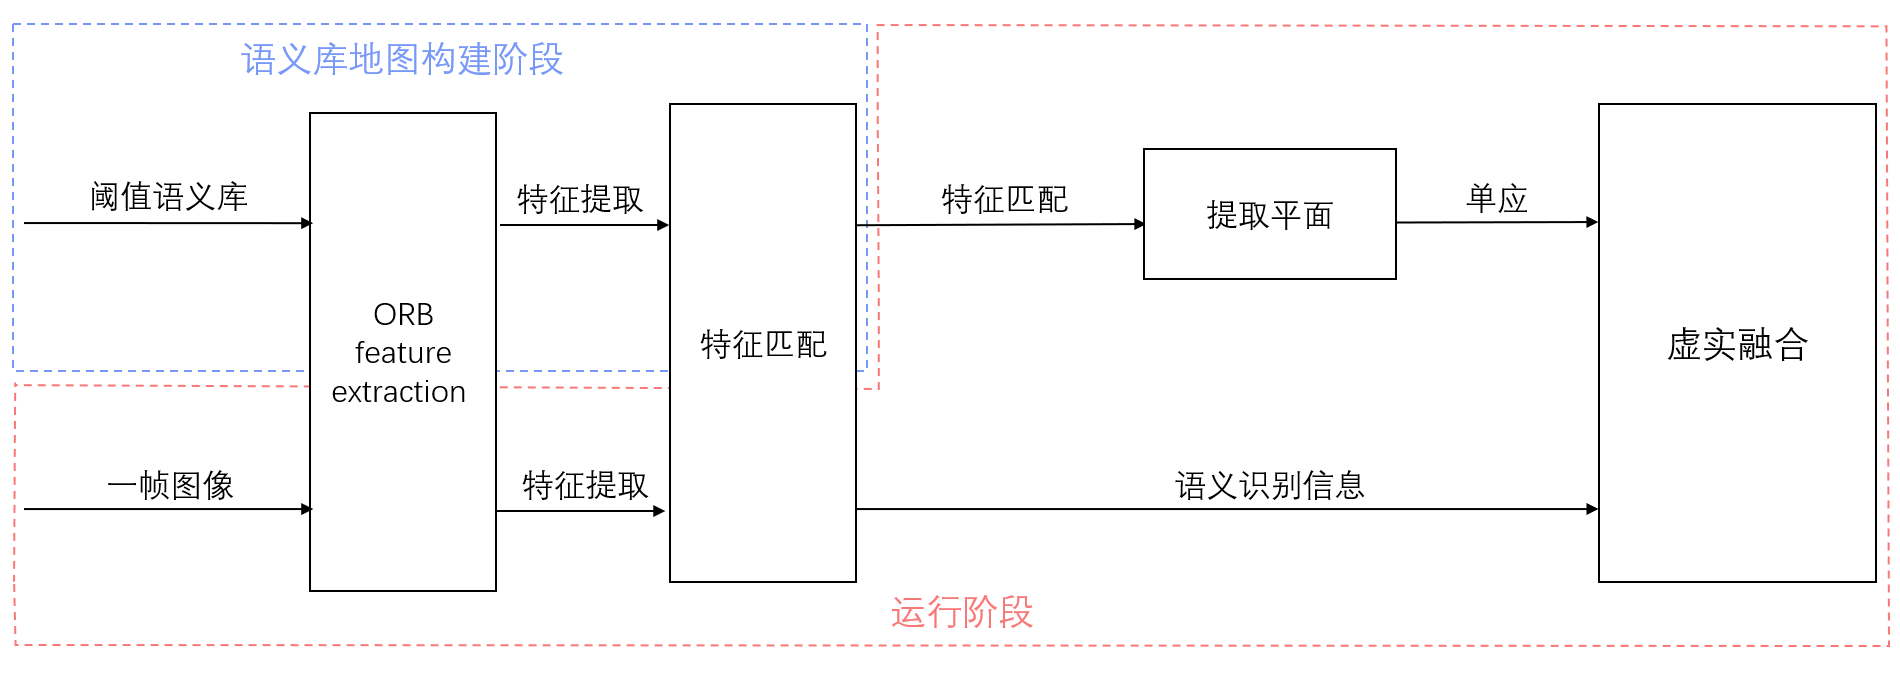
\includegraphics[width=0.5\textwidth]{Img/4-ismar.png}
    \bicaption{基于预置语义库地图的增强现实系统工作流程。}{Workflow of augmented reality system based on preset semantic library map.}
    \label{fig:ismar}
\end{figure}
对于一个已知的室外场景,我们预先取得其中标志性位置的图像,提取其中的特征点,构成预置语义库地图,因相比于SIFT或SURF,ORB特征点
能够达到实时的特征提取与匹配,同时具有较好的鲁棒性,因此,我们选择了ORB特征点构造预置语义库地图,表示为$\mathbb{M}=\left\{map_{0},...,map_{n}\right\}$,$map_{i}=\left[lng_{i},lat_{i},alt_{i},\mathbb{F}_{i}\right]$,
其中各项分别表示这一地图点的地理位置,包括经度、纬度和海拔,以及从这张图像中提取到的特征点集合。

在程序运行的过程中,系统实时通过设备内置的GPS获取当前的地理坐标,在$t$时刻表示为$cor_{t}=\left[lng_{t},lat_{t},alt_{t}\right]$,
同时,实时计算设备与$\mathbb{M}$各地图点的地理距离$dis_{ti}$,若与某一元素的距离小于一阈值$dis_{0}$,则认为当前设备进入了
此地图点的可视范围。

由于地图点可能分布较密集,其间距可能它小于GPS的精度,因此不能仅依靠以GPS坐标计算的设备与地图点的间距来识别地图点。在设备进入一
可是范围后,我们使用特征匹配的方法进行进一步精确的图像识别。具体来说,在进入一可视范围后,会对相机捕获的图像也提取ORB特征点,
与可视范围内的所有地图点存储的特征点集合进行匹配。对具有最高匹配相似度且高于一定阈值的地图点,认为当前设备所捕捉的图像正是
此地图点所存储的相应图像,系统可以从语义库中读取关于此位置的环境信息。

若连续两帧$F_{k-1}$、$F_{k}$匹配到了同一地图点,对这两帧图像的特征点$\mathbb{F}_{k-1}$、$\mathbb{F}_{k}$
,将仅保留与地图点特征点集相匹配的特征点,$\mathbb{F}_{k-1}^{'}$、$\mathbb{F}_{k}^{'}$,并对$\mathbb{F}_{k-1}^{'}$和$\mathbb{F}_{k}^{'}$
再次进行匹配,用匹配结果来计算对应环境平面的单应,得出相机坐标系到此地图点对应场景平面的转移矩阵。通过与地图点的特征匹配
保留下来的特征点,将是仅属于地图点对应场景平面的特征点,通过这些点之间的匹配关系计算的单应能够确保其唯一性,同时,因特征点数
的减少,程序运行开销也将降低。

具体的单应计算方法是,先通过RANSAC算法,从匹配点集中采用四个点对,计算单应矩阵初值$H_{0}$,之后通过最小化重投影误差,迭代
求得最优的单应:
$$H^{*}=\mathop{argmin}\limits_{H}\sum\limits_{i=1}^{n}\left \|f_{k}^{i}-Hf_{k-1}^{i} \right \|+\left \|f_{k-1}^{i}-H^{-1}f_{k}^{i} \right \|$$

根据以上方法,可以通过预先构造场景的预置语义库地图,通过结合GPS和特征识别的方法,识别设备所捕捉的图像并计算相机到场景平面的转移矩阵,获取对场景的语义理解。

\section{物体级语义地图的构建和表示}
\ref{cha_41}中介绍的基于局部特征的预置语义库地图需要预先构造语义库,仅能理解环境中少部分场景,没有在几何和语义层面对整个场景进行全面理解。SLAM系统
能够构造未知环境的几何地图,更好地全面理解并表示一个场景。然而传统基于特征的视觉SLAM系统构造的地图仅能表达几何空间结构,并且在
场景发生动态变化时会出现重影等问题。因此,本节研究了一种基于语义SLAM的物体级三维语义点云地图,能够结合对相机捕获的图像的实例级分割结果,
对其中物体分别建模并跟踪,为其赋予语义标签,并通过深度图像建立物体级的三维点云地图,给予场景高层的理解和表示。

\subsection{物体级语义点云地图生成方法}
在本文所提出的SLAM系统中,语义建图线程接受跟踪线程生成的关键帧$KF$和语义分割线程生成的关键帧的实例分割结果$\mathbb{R}$,
根据每一关键帧的信息增量式建图。语义建图线程处理一关键帧用时长于跟踪线程处理一帧的用时,为更好地利用计算资源,保证程序平滑运行,使得不同处理频率的线程同步进行,
我们创建了待处理关键帧队列$Q_{kf}$作为缓冲区,新生成的关键帧和相应的预测结果将插入$Q_{kf}$队尾,在处理过程中从将从队头取出。
\begin{figure}[!htbp]
    \centering
    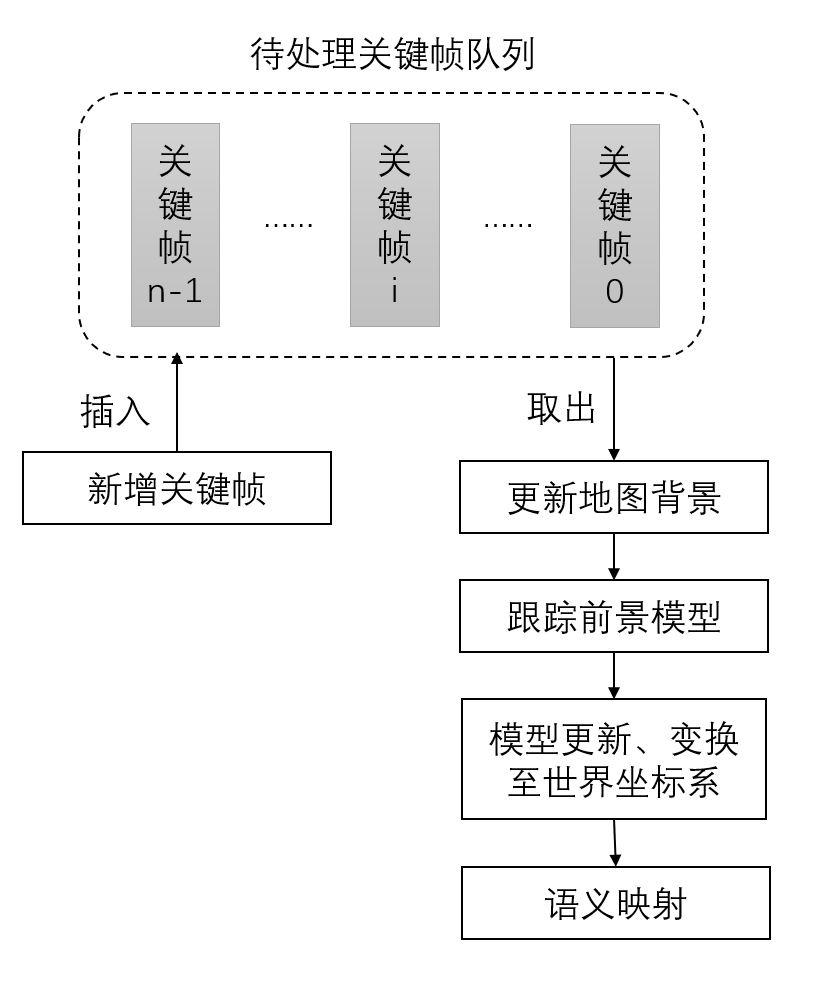
\includegraphics[width=\textwidth]{Img/4-queue.png}
    \bicaption{物体级语义建图模块工作流程。}{Object-level semantic mapping module workflow.}
    \label{fig:queue}
\end{figure}
本节研究的物体级语义地图由一个全局的背景模型$L_{0}$和一系列前景物体模型${L_{1},...,L_{i},...,L_{n}}$组成,前景物体模型将通过模型列表$\mathbb{L}$进行管理和维护。
其中$L_{i}=\left[\mathbb{PC}_{i}, cls_{i}, id_{i}, num_{i}, flag_{i} \right]$,各项表示此模型的点云模型、类别标签、模型编号、
连续跟踪丢失的帧数和成功跟踪标记。$\mathbb{PC}_{i}=\left[pc_{i}^{0},...,pc_{i}^{s},...,pc_{i}^{m}\right]$为一系列三维点集合,其中每个点表示为$pc_{i}^{s}=\left \{ x, y, z, b, g, r \right \}$,
分别为这一三维点在世界坐标系下的坐标和表示颜色的RGB分量。值得一提的是,对于全局背景模型$L_{0}$来说,它仅包含$\mathbb{PC}_{0}$和$id_{0}$两项。

建图过程中,系统增量式地更新$L_{0}$,为适应环境中目标的动态变化,会对$\mathbb{L}$中的模型进行跟踪,
为新检测到的物体建模、为跟踪到的物体模型更新、并删除跟踪丢失的模型。对每个关键帧完成模型跟踪后,将当前$\mathbb{L}$中可见的所有模型分别变换到
世界坐标系下的地图中,从而地图中物体模型随实现环境中物体移动而变化的效果。

下面以更新$L_{0}$为例,介绍增量式更新点云模型的方法。首先从$Q$队首取出关键帧$KF$和实例级分割结果$\mathbb{R}$,$KF$包括此帧的
彩色图$C$和深度图$D$。在$D$中,以一定步长间隔$step$取点,在实验中我们选取$step=3$,所取点$P=[u, v]$需满足:
\begin{equation} 
    \adddotsbeforeeqnnum%
    \begin{cases}
        m_{u,v}=0\\
        d_{min}<d<d_{max}\\
    \end{cases}
\end{equation}
即点$P$非前景目标,且深度值在一定范围内。其中$d=D(u,v)$,$d_{min}$和$d_{max}$为预设的深度阈值。

接下来通过相机内参$K$将$P$投影到相机坐标系下,得到点$X=[x,y,z]$:
\begin{equation} 
    \adddotsbeforeeqnnum%
    \begin{cases}
        x=\frac{u-cx}*d{fx}\\
        y=\frac{v-cy}*d{fy}\\
        z=d
    \end{cases}
\end{equation}

之后根据视觉里程计模块对此关键帧估计的位姿转移矩阵$T_{cw}$,将$X$变换至世界坐标系下,得到$\hat{X}$,即为对应点云模型中一点$pc$的
前三维分量。同时以彩色图上此点的r、g、b值$C(u,v)$作为$pc$的后三维分量:
\begin{equation} 
    \adddotsbeforeeqnnum%
    \begin{cases}
        pc_{0:2}=T_{cw}^{-1}\hat{X}\\
        pc_{3:5}=C(u,v)\\ 
    \end{cases}
\end{equation}

所有满足条件的点经处理后得到的三维点集合作为点云模型增量$L_{0}^{inv}$,用其更新$L_{0}$:
$$L_{0}=L_{0} \oplus L_{0}^{inv}$$
其中$\oplus$表示点云的融合相加操作。

前景模型的跟踪与之相似,不同之处为,对一个前景模型$L_{i}$和相应目标检测结果$r_{j}$,其选点需满足的条件为:
\begin{equation} 
    \adddotsbeforeeqnnum%
    \begin{cases}
        w_{m_{u,v}}=c_{j}\\
        d_{min}<d<d_{max}\\
        bu_{j}\geq u\geq bu_{j}+bw_{j}\\
        bv_{j}\geq v\geq bv_{j}+bh_{j}\\
    \end{cases}
\end{equation}
即点$P$为$r_{j}$的一前景点,且其深度在对应范围内。

此外,在生成三维点云时的步骤也有所不同,对于前景模型,将根据其类别$cls_{i}$选取对应颜色作为$pc$的后三维分量,点云地图
中各物体不同的颜色表示其不同的物体类别。

\subsection{物体建模和跟踪方法}

本研究的模型跟踪策略基于以下两个观察:
{
\setlist[enumerate]{}% restore default behavior
\begin{enumerate}[nosep]
    \item 对于一个运动中的物体,尤其是非刚体运动,比如人的挥手动作,增量式更新前景目标模型会导致形变局部产生重影。
    \item 对于静态的前景物体,其在连续关键帧之间的坐标位置不会有跳跃性的改变,而在局部遮挡、视野缺失等情况下容易跟踪失败。
\end{enumerate}
}
因此,我们提出了基于物体运动类别的模型跟踪策略。
对动态前景目标和静态前景目标,设置了不同的跟踪阈值$TT_moving$、$TT_static$和丢失阈值$TL_moving$、$TL_static$,
分别表示跟踪成功的最小IoU和跟踪丢失的最小连续帧数。
在程序运行阶段,对于检测到的一个物体$r_{j}$,首先根据其类别判定是否可能处于运动状态,若$w_{c_{j}}>0$,则认为此目标是一个
动态前景目标,反之认为此目标是一个静态前景目标,然后根据目标的运动类别选择相应的跟踪阈值和丢失阈值。一个模型的跟踪成功与否,
依靠当前关键帧检测到的个目标与其重合程度来计算,本研究使用了连续两关键帧上轮廓的IoU表示,IoU越大可能意味着此目标发生运动,或视野缺失。
对于动态前景目标,发生移动后应倾向于对其重新建模,以避免运动而产生的模型重影,因此其跟踪条件更为严格。
对于静态前景目标,发生移动后应倾向于对其进行维护,以避免因视野确实而造成的跟踪丢失,因此其跟踪条件更为宽松。

我们保存了上一个关键帧的语义mask$m_{pre}$和检测结果$\mathbb{R}_{pre}$,
对于当前关键帧检测到的目标,在跟踪过程中使用$\mathbb{L}$中同类别模型的语义mask和当前目标的语义mask计算IoU,根据IoU判定与模型的相似度。
直接在语义分割模块预测得到的2D语义mask上计算IoU,能够避免将模型投影到当前关键帧带来的大量计算开销。
而根据运动状态选择不同跟踪判断阈值,也能弥补相机视角变化带来的误差,从而使得跟踪过程具有较高的鲁棒性和准确度。

程序运行过程中,对于一个目标检测结果$r_{j}$,首先获取$\mathbb{L}$中与其同类别且未被跟踪到的模型集合$\mathbb{L}_{j}$,若此集合为空,
则为$r_{j}$新建一个模型插入模型列表,否则,使用$\mathbb{L}_{j}$的中模型依次与$r_{j}$计算IoU,得到最大的IoU和对应模型$MaxIoU, MaxL$。
之后,根据$MaxL$的先验权重$w_{cls_{MaxL}}$,判断其为动态前景目标还是静态前景目标,获取其对应的跟踪阈值$TT_{MaxL}$,若$MaxIoU$大于$TT_{MaxL}$,
则认为$MaxL$与$r_{j}$相匹配,跟踪成功,根据$r_{j}$计算点云模型增量,用以更新$\mathbb{PC}_{MaxL}$,更新此模型的连续跟踪失败帧数$num_{MaxL}$为0,设置跟踪成功标记$flag_{MaxL}$为真。否则,为$r_{j}$新建一个模型插入模型列表。
处理完所有检测到的目标的后,遍历$\mathbb{L}$中所有模型$L_{i}$,对于跟踪成功标记为假的模型,将其连续跟踪失败帧数加一。
之后,再次遍历$\mathbb{L}$中所有模型$L_{i}$,根据$MaxL$的先验权重$w_{cls_{i}}$,判断其为动态前景目标还是静态前景目标,获取其对应的丢失阈值$TL_{i}$,
若该模型的连续跟踪失败帧数$num_{i}$大于$TL_{i}$,则认为此模型跟丢,从模型列表中删除。

此算法具体描述为:
\begin{algorithm} %算法开始 
    \small
    \caption{模型跟踪算法} \label{alg1} %算法的标签 
    \begin{algorithmic}[1] %此处的[1]控制一下算法中的每句前面都有标号 
    \Procedure{跟踪后的模型列表}{$L^{'}$}
    \For{each $r_{j}$ in $\mathbb{R}$}
        \State $\mathbb{L}_{j}\gets GetModelInSameCategory(\mathbb{L},c_{j})$
        \If{$\mathbb{L}_{j}$ is empty}
            \State $L^{'}\gets BuildNewModel(r_{j})$
        \Else
            \For{each $L_{i}$ in $\mathbb{L}_{j}$}
                \State $IoU_{i,j}\gets CalIoU(m_{pre},\mathbb{R}_{pre},m,r_{j})$
                \State $MaxIoU, MaxL\gets UpdateClosestModel(IoU_{i,j},L_{i},MaxIoU, MaxL)$
            \EndFor
            \State $TT_{MaxL}\gets GetIoUThreshold(w_{cls_{MaxL}},TT_moving、TT_static)$
            \If{$MaxIou>TT_{MaxL}$}
                \State $L^{'}\gets UpdateModel(r_{j},MaxL)$
                \State $num_{MaxL}\gets 0$
                \State $flag_{MaxL}\gets true$
            \Else
                \State $L^{'}\gets BuildNewModel(r_{j})$
            \EndIf
        \EndIf
    \EndFor
    \For{each $L_{i}$ in $\mathbb{L}_{j}$}
        \If{$flag_{i} is false$}
            \State $num_{i}\gets num_{i}+1$
        \EndIf
    \EndFor
    \For{each $L_{i}$ in $\mathbb{L}_{j}$}
        \State $TL_{i}\gets GetLostThreshold(cls_{i},TL_moving、TL_static)$
        \If{$num_{i}>TL_{i}$}
            \State $L^{'}\gets DeleteModel(L_{i})$
        \EndIf
    \EndFor
    \EndProcedure
    \end{algorithmic} 
\end{algorithm}

\section{实验结果与分析}
我们使用TUM RGB-D数据集中高度动态的片段\emph{walking\_xyz}来测试了物体级语义地图的构建和表示效果。\ref{fig:maps}展示了在
第63帧和第87帧,原彩色图、深度图、实例分割结果和物体级语义建图结果图。可以看出,经实例分割得出的前景目标都被单独建模显示在了
三维点云地图的正确中,并且被赋予了不同颜色,以表示其类别。这里,蓝色表示类别“人”,红色表示类别“显示器”,紫色表示类别“椅子”,
黄色表示类别“水杯”。此外,在第63帧和第87帧直接,场景中人物发生了移动,而三维地图中对应模型也进行了相应更新。

\begin{figure}[!htbp]
    \centering
    \begin{subfigure}[b]{0.35\textwidth}
      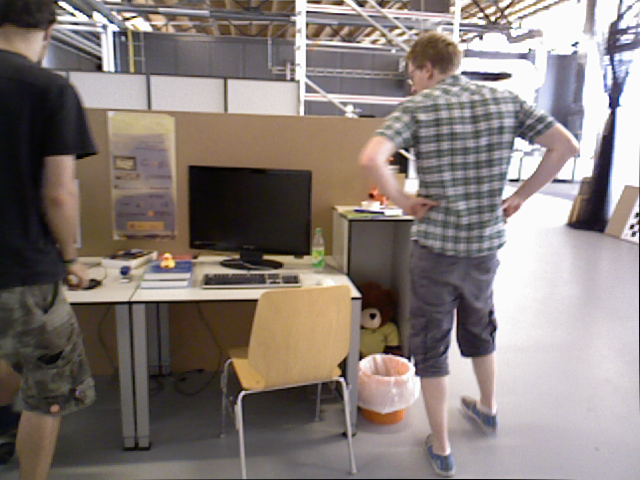
\includegraphics[width=\textwidth]{Img/ori_63.png}
      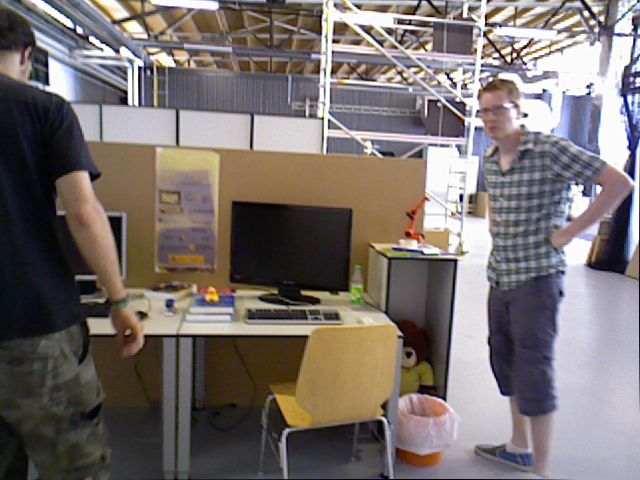
\includegraphics[width=\textwidth]{Img/ori_87.png}
      \caption{}
      \label{fig:ori}
    \end{subfigure}%
    \begin{subfigure}[b]{0.35\textwidth}
      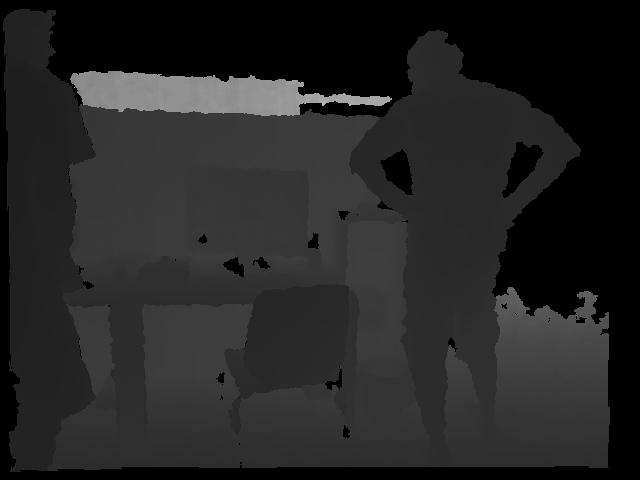
\includegraphics[width=\textwidth]{Img/depth_63.png}
      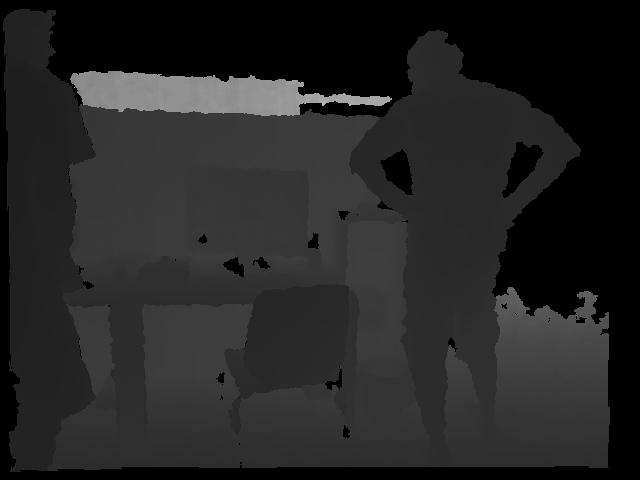
\includegraphics[width=\textwidth]{Img/depth_63.png}
      \caption{}
      \label{fig:depth}
    \end{subfigure}%
    ~% add desired spacing
    \\% line break
    \begin{subfigure}[b]{0.35\textwidth}
        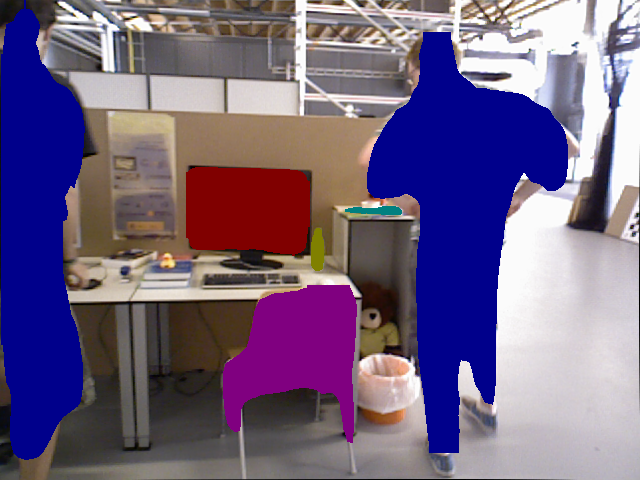
\includegraphics[width=\textwidth]{Img/mask_63.png}
        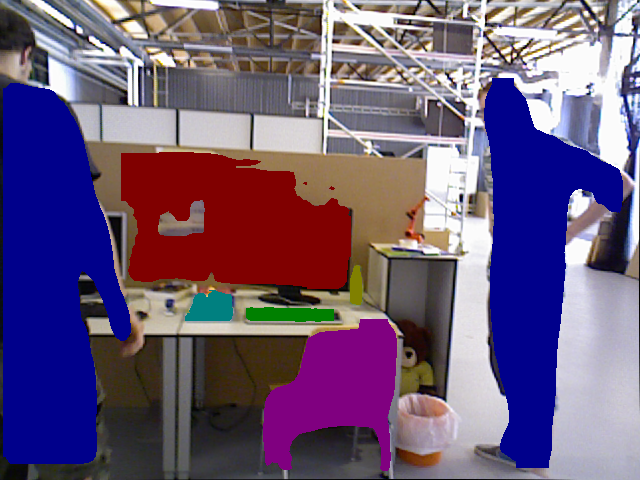
\includegraphics[width=\textwidth]{Img/mask_87.png}
      \caption{}
      \label{fig:mask}
    \end{subfigure}%
    ~% add desired spacing
    \begin{subfigure}[b]{0.35\textwidth}
        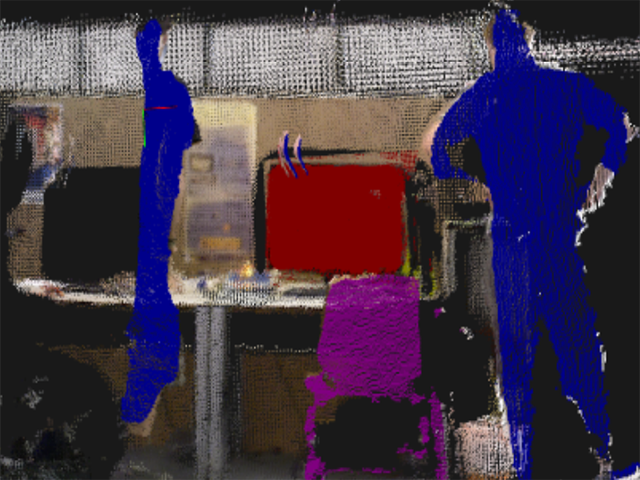
\includegraphics[width=\textwidth]{Img/map_63.png}
        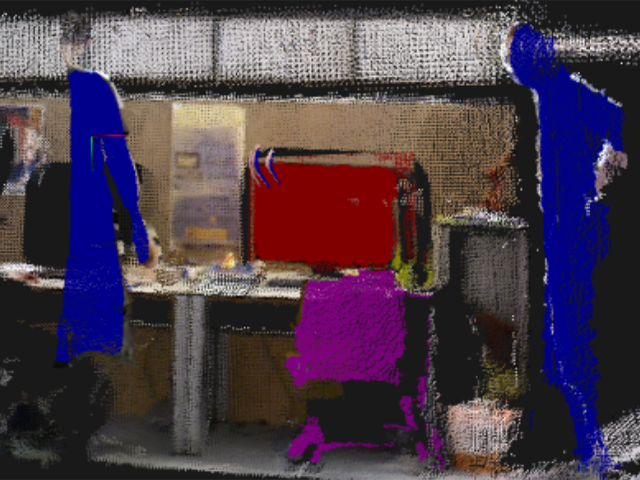
\includegraphics[width=\textwidth]{Img/map_87.png}
      \caption{}
      \label{fig:map}
    \end{subfigure}
    \bicaption{\emph{walking\_xyz}序列第63帧和第87帧的建图效果。(a) 原彩色图,(b) 原深度图,(c) 实例分割结果,(c) 物体级语义建图效果。}{ Illustration of our experimental results for frame 63 and frame 87 in sequence \emph{walking\_xyz}. 
    (a) the raw RGB image, (a) the raw depth image, (c)instance-level segmentation results, (c)object-aware semantic point cloud map.}
    \label{fig:maps}
\end{figure}
  
然而当前物体级语义地图构建和表示方法仍存在一些问题,比如地图中物体边缘不够精准,存在比较多的黑色孔洞等,需要在之后的工作中完善。

\section{本章小结}
本章按照不同的语义表达方式,讨论了两种语义地图的构建和表示方法。首先介绍了基于局部特征的预置语义库地图的构建和表示方法,
之后介绍了基于语义SLAM的物体级三维语义点云地图的构建和表示方法。这二者分别侧重于室外场景和动态场景,都能够一定程度上对于环境在语义层面上进行表达,从而用于增强显示应用的虚实融合方法优化。
在基于语义SLAM的物体级三维语义点云地图的构建方面,本章还详述了其在动态环境根据目标类别而指定物体跟踪策略。
最后给出了物体级三维语义点云地图的建图效果图,对实验结果进行了分析。
\chapter{增强现实原型系统的设计与实现}\label{chap:5}
\section{基于语义地图的虚实融合方法研究}
\section{增强现实原型系统设计}
\section{实验结果与分析}
\section{本章小结}

\chapter{总结与展望}\label{chap:6}
\section{研究总结}
增强现实是一种当今社会中高速发展的新兴技术,丰富多彩增强现实应用正在逐渐进入人们的娱乐、学习、生产等领域。虚实融合技术是增强现实
领域的关键技术之一,它通过跟踪相机自身位姿,将虚拟资料注册在显示环境中的恰当位置。虚实融合效果的好坏能够影响增强现实系统在
物理遮挡问题等方面的表现,从而影响系统的真实性体验。基于特征的视觉SLAM技术能一定程度上解决相机位姿估计和环境几何信息理解的问题,从而帮助虚实融合,
但在动态环境下的位姿估计和建图、语义信息表达等方面仍有不足。本文针对以上问题,构建了结合深度神经网络和视觉SLAM框架的语义SLAM系统,
对于对动态场景下位姿估计优化方法、语义地图的构建和表示方法及在增强现实系统中的应用方法进行了研究。本文的主要工作和贡献如下:
{
\setlist[enumerate]{}% restore default behavior
\begin{enumerate}[nosep]
    \item 动态场景下基于语义信息的位姿估计优化方法\\这部分研究工作针对动态场景,提出了双阶段的动态外点滤除算法,此算法结合基于语义类别的
    自适应权重生成方法和基于极线约束的动态一致性检测方法,能够对于不同类别的物体自适应生成不同的判定条件,判断其是否处于运动状态,
    并移除处于运动状态的物体的轮廓内的特征点。此算法在TUM RGB-D数据集上进行了验证,在动态场景下其结果比ORB-SLAM2有数量级式的提升,
    提升幅度在大部分指标上优于业界先进系统,表明它能够有效减少环境中运动物体对于SLAM系统位姿估计的干扰,提升基于特征的视觉SLAM系统在动态场景下的位姿估计精度和鲁棒性。
    \item 语义地图的构建和表示方法\\这部分研究工作针对不同层级语义地图对环境的表示能力,分别探究了基于局部特征的预置语义库地图和语义SLAM系统生成的
    物体级三维语义点云地图的构建和表示方法。对于预置语义库地图提出了特征识别和跟踪方法,验证了其对室外环境的表示能力和在增强现实导航系统中的应用能力。
    对于物体级三维语义点云地图,本文提出了针对语义类别的物体跟踪策略,能够对环境中的物体分别建模、跟踪,适应动态变化的环境,并进行语义关联。
    此方法在动态环境和静态环境下分别进行了验证,结果表明它能够提高建图的鲁棒性,建立随环境变化而变化的物体级语义地图,从而提高对三维环境的表示能力。
    \item 增强现实原型系统的设计与实现\\这部分研究工作设计并实现了一个增强现实原型系统,融合了述研究的算法,在虚实融合阶段进行了
    优化,提升了系统的真实感体验。
\end{enumerate}
}

\section{未来展望}
增强现实技术是当前最有研究前景和应用价值的技术之一,各大高校、公司和研究机构都有相关的研究战略部署,如微软公司发布的HoloLens平台、
苹果公司发布的ARKit平台、谷歌公司发布的ARCore平台、高通公司发布的Vuforia平台等,都取得了不俗的表现,也拥有很大的发展空间。
本文研究的基于语义SLAM的增强现实虚实融合关键技术,虽然一定程度上提高了系统在动态环境下位姿估计精度,建立了物体级的三维语义地图,
但仍存在一些局限,仍需在未来工作中探究。具体的未来研究方向有:
{
\setlist[enumerate]{}% restore default behavior
\begin{enumerate}[nosep]
    \item 系统实时性较低\\当前系统受限于语义分割模块对图像的处理速度过慢,无法取得实时运行的效果,这限制了基于此系统的增强现实
    应用在实际环境中的应用。在未来的工作中,可以尝试使用更高效的实例分割网络结构,或按照一定策略间隔取帧进行实例分割,以取得
    位姿估计精度和运行效率的平衡。
    \item 静态环境下位姿估计提升效果不显著\\当前系统通过检测场景中的动态目标,滤除其轮廓内的特征点的方法,来减少动态环境对
    相机位姿估计的影响,但这种方法在静态环境或低动态环境下对位姿估计的提升效果并不显著。其原因之一是当前基于光流的动态一致性
    检测方法对光照等环境变化敏感,容易造成误判,经特征点滤除之后,图像中用于迭代、优化的特征点总数减少。在未来的工作中,
    可以尝试使用其他物体移动的检测方法,以更精确地滤除动态特征点。
    \item 模型精度不足\\当前语义建图模块所建的物体级语义地图的模型仍比较粗糙,存在边缘模糊、部分缺失的情况。主要原因是实例分割
    模块输出的语义mask边缘不够精细,在发生物理遮挡、视野部分丢失的情况时,也会导致建模不完整。在未来的工作中,可以尝试结合
    基于几何特性的分割方法,在二维图像或三维点云上进行物体边缘分割,以细化语义分割模块实例分割的结果。还可以使用能够支持物体形变
    的建模方法,在更长的时间跨度上对模型进行跟踪和维护。
    
\end{enumerate}
}

%---------------------------------------------------------------------------%

% main content
%-
%-> Appendix
%-
% \cleardoublepage%
% \appendix% initialize the environment
% \chapter{中国科学院大学学位论文撰写要求}

学位论文是研究生科研工作成果的集中体现,是评判学位申请者学术水平、授予其学位的主要依据,是科研领域重要的文献资料。根据《科学技术报告、学位论文和学术论文的编写格式》(GB/T 7713-1987)、《学位论文编写规则》(GB/T 7713.1-2006)和《文后参考文献著录规则》(GB7714—87)等国家有关标准,结合中国科学院大学(以下简称“国科大”)的实际情况,特制订本规定。

\section{论文无附录者无需附录部分}

\section{测试公式编号 \texorpdfstring{$\Lambda,\lambda,\theta,\bar{\Lambda},\sqrt{S_{NN}}$}{$\textLambda,\textlambda,\texttheta,\bar{\textLambda},\sqrt{S_{NN}}$}} \label{sec:testmath}

\begin{equation} \label{eq:appedns}
    \adddotsbeforeeqnnum%
    \begin{cases}
        \frac{\partial \rho}{\partial t} + \nabla\cdot(\rho\Vector{V}) = 0\\
        \frac{\partial (\rho\Vector{V})}{\partial t} + \nabla\cdot(\rho\Vector{V}\Vector{V}) = \nabla\cdot\Tensor{\sigma}\\
        \frac{\partial (\rho E)}{\partial t} + \nabla\cdot(\rho E\Vector{V}) = \nabla\cdot(k\nabla T) + \nabla\cdot(\Tensor{\sigma}\cdot\Vector{V})
    \end{cases}
\end{equation}
\begin{equation}
    \adddotsbeforeeqnnum%
    \frac{\partial }{\partial t}\int\limits_{\Omega} u \, \mathrm{d}\Omega + \int\limits_{S} \unitVector{n}\cdot(u\Vector{V}) \, \mathrm{d}S = \dot{\phi}
\end{equation}
\[
    \begin{split}
        \mathcal{L} \{f\}(s) &= \int _{0^{-}}^{\infty} f(t) e^{-st} \, \mathrm{d}t, \ 
        \mathscr{L} \{f\}(s) = \int _{0^{-}}^{\infty} f(t) e^{-st} \, \mathrm{d}t\\
        \mathcal{F} {\bigl (} f(x+x_{0}) {\bigr )} &= \mathcal{F} {\bigl (} f(x) {\bigr )} e^{2\pi i\xi x_{0}}, \ 
        \mathscr{F} {\bigl (} f(x+x_{0}) {\bigr )} = \mathscr{F} {\bigl (} f(x) {\bigr )} e^{2\pi i\xi x_{0}}
    \end{split}
\]

mathtext: $A,F,L,2,3,5,\sigma$, mathnormal: $A,F,L,2,3,5,\sigma$, mathrm: $\mathrm{A,F,L,2,3,5,\sigma}$.

mathbf: $\mathbf{A,F,L,2,3,5,\sigma}$, mathit: $\mathit{A,F,L,2,3,5,\sigma}$, mathsf: $\mathsf{A,F,L,2,3,5,\sigma}$.

mathtt: $\mathtt{A,F,L,2,3,5,\sigma}$, mathfrak: $\mathfrak{A,F,L,2,3,5,\sigma}$, mathbb: $\mathbb{A,F,L,2,3,5,\sigma}$.

mathcal: $\mathcal{A,F,L,2,3,5,\sigma}$, mathscr: $\mathscr{A,F,L,2,3,5,\sigma}$, boldsymbol: $\boldsymbol{A,F,L,2,3,5,\sigma}$.

vector: $\Vector{\sigma, T, a, F, n}$, unitvector: $\unitVector{\sigma, T, a, F, n}$

matrix: $\Matrix{\sigma, T, a, F, n}$, unitmatrix: $\unitMatrix{\sigma, T, a, F, n}$

tensor: $\Tensor{\sigma, T, a, F, n}$, unittensor: $\unitTensor{\sigma, T, a, F, n}$ 

\section{测试生僻字}

霜蟾盥薇曜灵霜颸妙鬘虚霩淩澌菀枯菡萏泬寥窅冥毰毸濩落霅霅便嬛岧峣瀺灂姽婳愔嫕飒纚棽俪緸冤莩甲摛藻卮言倥侗椒觞期颐夜阑彬蔚倥偬澄廓簪缨陟遐迤逦缥缃鹣鲽憯懔闺闼璀错媕婀噌吰澒洞阛闠覼缕玓瓑逡巡諓諓琭琭瀌瀌踽踽叆叇氤氲瓠犀流眄蹀躞赟嬛茕頔璎珞螓首蘅皋惏悷缱绻昶皴皱颟顸愀然菡萏卑陬纯懿犇麤掱暒 墌墍墎墏墐墒墒墓墔墕墖墘墖墚墛坠墝增墠墡墢墣墤墥墦墧墨墩墪樽墬墭堕墯墰墱墲坟墴墵垯墷墸墹墺墙墼墽垦墿壀壁壂壃壄壅壆坛壈壉壊垱壌壍埙壏壐壑壒压壔壕壖壗垒圹垆壛壜壝垄壠壡坜壣壤壥壦壧壨坝塆圭嫶嫷嫸嫹嫺娴嫼嫽嫾婳妫嬁嬂嬃嬄嬅嬆嬇娆嬉嬊娇嬍嬎嬏嬐嬑嬒嬓嬔嬕嬖嬗嬘嫱嬚嬛嬜嬞嬟嬠嫒嬢嬣嬥嬦嬧嬨嬩嫔嬫嬬奶嬬嬮嬯婴嬱嬲嬳嬴嬵嬶嬷婶嬹嬺嬻嬼嬽嬾嬿孀孁孂娘孄孅孆孇孆孈孉孊娈孋孊孍孎孏嫫婿媚嵭嵮嵯嵰嵱嵲嵳嵴嵵嵶嵷嵸嵹嵺嵻嵼嵽嵾嵿嶀嵝嶂嶃崭嶅嶆岖嶈嶉嶊嶋嶌嶍嶎嶏嶐嶑嶒嶓嵚嶕嶖嶘嶙嶚嶛嶜嶝嶞嶟峤嶡峣嶣嶤嶥嶦峄峃嶩嶪嶫嶬嶭崄嶯嶰嶱嶲嶳岙嶵嶶嶷嵘嶹岭嶻屿岳帋巀巁巂巃巄巅巆巇巈巉巊岿巌巍巎巏巐巑峦巓巅巕岩巗巘巙巚帠帡帢帣帤帨帩帪帬帯帰帱帲帴帵帷帹帺帻帼帽帾帿幁幂帏幄幅幆幇幈幉幊幋幌幍幎幏幐幑幒幓幖幙幚幛幜幝幞帜幠幡幢幤幥幦幧幨幩幪幭幮幯幰幱庍庎庑庖庘庛庝庠庡庢庣庤庥庨庩庪庬庮庯庰庱庲庳庴庵庹庺庻庼庽庿廀厕廃厩廅廆廇廋廌廍庼廏廐廑廒廔廕廖廗廘廙廛廜廞庑廤廥廦廧廨廭廮廯廰痈廲廵廸廹廻廼廽廿弁弅弆弇弉弖弙弚弜弝弞弡弢弣弤弨弩弪弫弬弭弮弰弲弪弴弶弸弻弼弽弿彖彗彘彚彛彜彝彞彟彴彵彶彷彸役彺彻彽彾佛徂徃徆徇徉后徍徎徏径徒従徔徕徖徙徚徛徜徝从徟徕御徢徣徤徥徦徧徨复循徫旁徭微徯徰徱徲徳徴徵徶德徸彻徺忁忂惔愔忇忈忉忔忕忖忚忛応忝忞忟忪挣挦挧挨挩挪挫挬挭挮挰掇授掉掊掋掍掎掐掑排掓掔掕挜掚挂掜掝掞掟掠采探掣掤掦措掫掬掭掮掯掰掱掲掳掴掵掶掸掹掺掻掼掽掾掿拣揁揂揃揅揄揆揇揈揉揊揋揌揍揎揑揓揔揕揖揗揘揙揤揥揦揧揨揫捂揰揱揲揳援揵揶揷揸揻揼揾揿搀搁搂搃搄搅搇搈搉搊搋搌搎搏搐搑搒摓摔摕摖摗摙摚摛掼摝摞摠摡斫斩斮斱斲斳斴斵斶斸旪旫旮旯晒晓晔晕晖晗晘晙晛晜晞晟晠晡晰晣晤晥晦晧晪晫晬晭晰晱晲晳晴晵晷晸晹晻晼晽晾晿暀暁暂暃暄暅暆暇晕晖暊暋暌暍暎暏暐暑暒暓暔暕暖暗旸暙暚暛暜暝暞暟暠暡暣暤暥暦暧暨暩暪暬暭暮暯暰昵暲暳暴暵
% appendix content
%-
%-> Backmatter: bibliography, glossary, index
%-
\backmatter% initialize the environment
\intotoc*{\cleardoublepage}{\bibname}% add link to toc
\bibliography{Biblio/ref}% bibliography
%---------------------------------------------------------------------------%
%->> Backmatter
%---------------------------------------------------------------------------%
\chapter{作者简历及攻读学位期间发表的学术论文与研究成果}

\textbf{本科生无需此部分}。

\section*{作者简历}


张琪,女,1995年出生,黑龙江省鸡西市人,汉族。2013年8月进入北京理工大学软件学院软件工程专业学习,2017年6月获得学士学位。
2017年9月进入中国科学院⾃动化研究所综合信息系统研究中⼼,攻读硕⼠学位,主要研究⽅向是虚拟现实与计算机图形学。

\section{联系方式}
通讯地址:北京市海淀区中关村东路95号

邮编:100190

E-mail: zhangqi2017@ia.ac.cn

\section*{已发表(或正式接受)的学术论文:}

{
\setlist[enumerate]{}% restore default behavior
\begin{enumerate}[nosep]
    \item Q. Zhang, X. Zhu, H. Yu and Y. Jiang, 
    Enhancing Rock Painting Tour Experience with Outdoor Augmented Reality, 
    submitted to 2019 IEEE International Symposium on Mixed and Augmented Reality Adjunct (ISMAR-Adjunct), 2019.
    (CCF B 类会议, Published)
\end{enumerate}
}

\section*{申请或已获得的专利:}

(无专利时此项不必列出)

\section*{攻读学位期间获奖情况}

\section*{攻读学位期间项目参与情况}


\chapter[致谢]{致\quad 谢}\chaptermark{致\quad 谢}% syntax: \chapter[目录]{标题}\chaptermark{页眉}
\thispagestyle{noheaderstyle}% 如果需要移除当前页的页眉
%\pagestyle{noheaderstyle}% 如果需要移除整章的页眉



\cleardoublepage[plain]% 让文档总是结束于偶数页,可根据需要设定页眉页脚样式,如 [noheaderstyle]
%---------------------------------------------------------------------------%
% other information
\end{document}
%---------------------------------------------------------------------------%

